\documentclass[sigconf]{styling/acmart}
%% NOTE that a single column version may required for 
%% submission and peer review. This can be done by changing
%% the \doucmentclass[...]{acmart} in this template to 
%% \documentclass[manuscript,screen]{acmart}
%% 
%% To ensure 100% compatibility, please check the white list of
%% approved LaTeX packages to be used with the Master Article Template at
%% https://www.acm.org/publications/taps/whitelist-of-latex-packages 
%% before creating your document. The white list page provides 
%% information on how to submit additional LaTeX packages for 
%% review and adoption.
%% Fonts used in the template cannot be substituted; margin 
%% adjustments are not allowed.

\usepackage{styling/additional_dependencies} % Bring in all the includes and Latex Utils

%%
%% \BibTeX command to typeset BibTeX logo in the docs
\AtBeginDocument{%
  \providecommand\BibTeX{{%
    \normalfont B\kern-0.5em{\scshape i\kern-0.25em b}\kern-0.8em\TeX}}}

\begin{document}
    % Everything prior to the main body of content

% Tell TexCount to ignore words in word count
%TC:ignore
% \pagenumbering{gobble} % Don't track page numbers prior to Table of Contents
% \thispagestyle{empty} % Remove Page Styling prior to Table of Contents
% \newgeometry{inner=0.2\textwidth,outer=0.2\textwidth}

%% Rights management information.  This information is sent to you
%% when you complete the rights form.  These commands have SAMPLE
%% values in them; it is your responsibility as an author to replace
%% the commands and values with those provided to you when you
%% complete the rights form.
\setcopyright{acmcopyright}
% \copyrightyear{2018}
% \acmYear{2018}
\acmDOI{XXXXXXX.XXXXXXX}

%% These commands are for a PROCEEDINGS abstract or paper.
\acmConference[Conference acronym 'XX]{}{N/A}{N/A}
%
%  Uncomment \acmBooktitle if th title of the proceedings is different
%  from ``Proceedings of ...''!
%
%\acmBooktitle{Woodstock '18: ACM Symposium on Neural Gaze Detection,
%  June 03--05, 2018, Woodstock, NY} 
% \acmPrice{}
% \acmISBN{}

% Setup title
\title{Distinguishing Between Head and Phone Gestures On a Smartphone With Front-Facing Camera and IMU}
% \renewcommand\maketitlehookb{\centering \Large }
\date{\today}
\author{James Whiffing} % Presume should also list supervisors here, but need to indicate?
% \authornote{}
\email{jw204@bath.ac.uk}
% \orcid{1234-5678-9012}
\affiliation{%
  \institution{University of Bath - Department of Computer Science}
%   \streetaddress{P.O. Box 1212}
  \city{Bath}
  \country{England}
%   \postcode{43017-6221}
}
%%
%% By default, the full list of authors will be used in the page
%% headers. Often, this list is too long, and will overlap
%% other information printed in the page headers. This command allows
%% the author to define a more concise list
%% of authors' names for this purpose.
\renewcommand{\shortauthors}{Whiffing, James}

%%
%% The abstract is a short summary of the work to be presented in the
%% article.
\begin{abstract}
    Head gesture recognition is a common approach taken in active research for increasing the available modes of input for mobile devices.
    Head tracking techniques that utilise the front-facing camera can incorrectly detect head movement caused by the phone being moved.
    In this work we review the mobile device head gesture recognition space to understand the techniques currently in-use. 
    We also perform a study with to collect head and phone movement data when performing semaphoric head and phone gestures. 
    We also propose a model/approach with which semaphoric head and phone gestures can be distinguished.
\end{abstract}

%%
%% The code below is generated by the tool at http://dl.acm.org/ccs.cfm.
%% Please copy and paste the code instead of the example below.
%%
\begin{CCSXML}

\end{CCSXML}

% \ccsdesc[500]{Computer systems organization~Embedded systems}
% \ccsdesc[300]{Computer systems organization~Redundancy}
% \ccsdesc{Computer systems organization~Robotics}
% \ccsdesc[100]{Networks~Network reliability}

%%
%% Keywords. The author(s) should pick words that accurately describe
%% the work being presented. Separate the keywords with commas.
% \keywords{} % TODO

%% A "teaser" image appears between the author and affiliation
%% information and the body of the document, and typically spans the
%% page.
\begin{teaserfigure}
  \center
  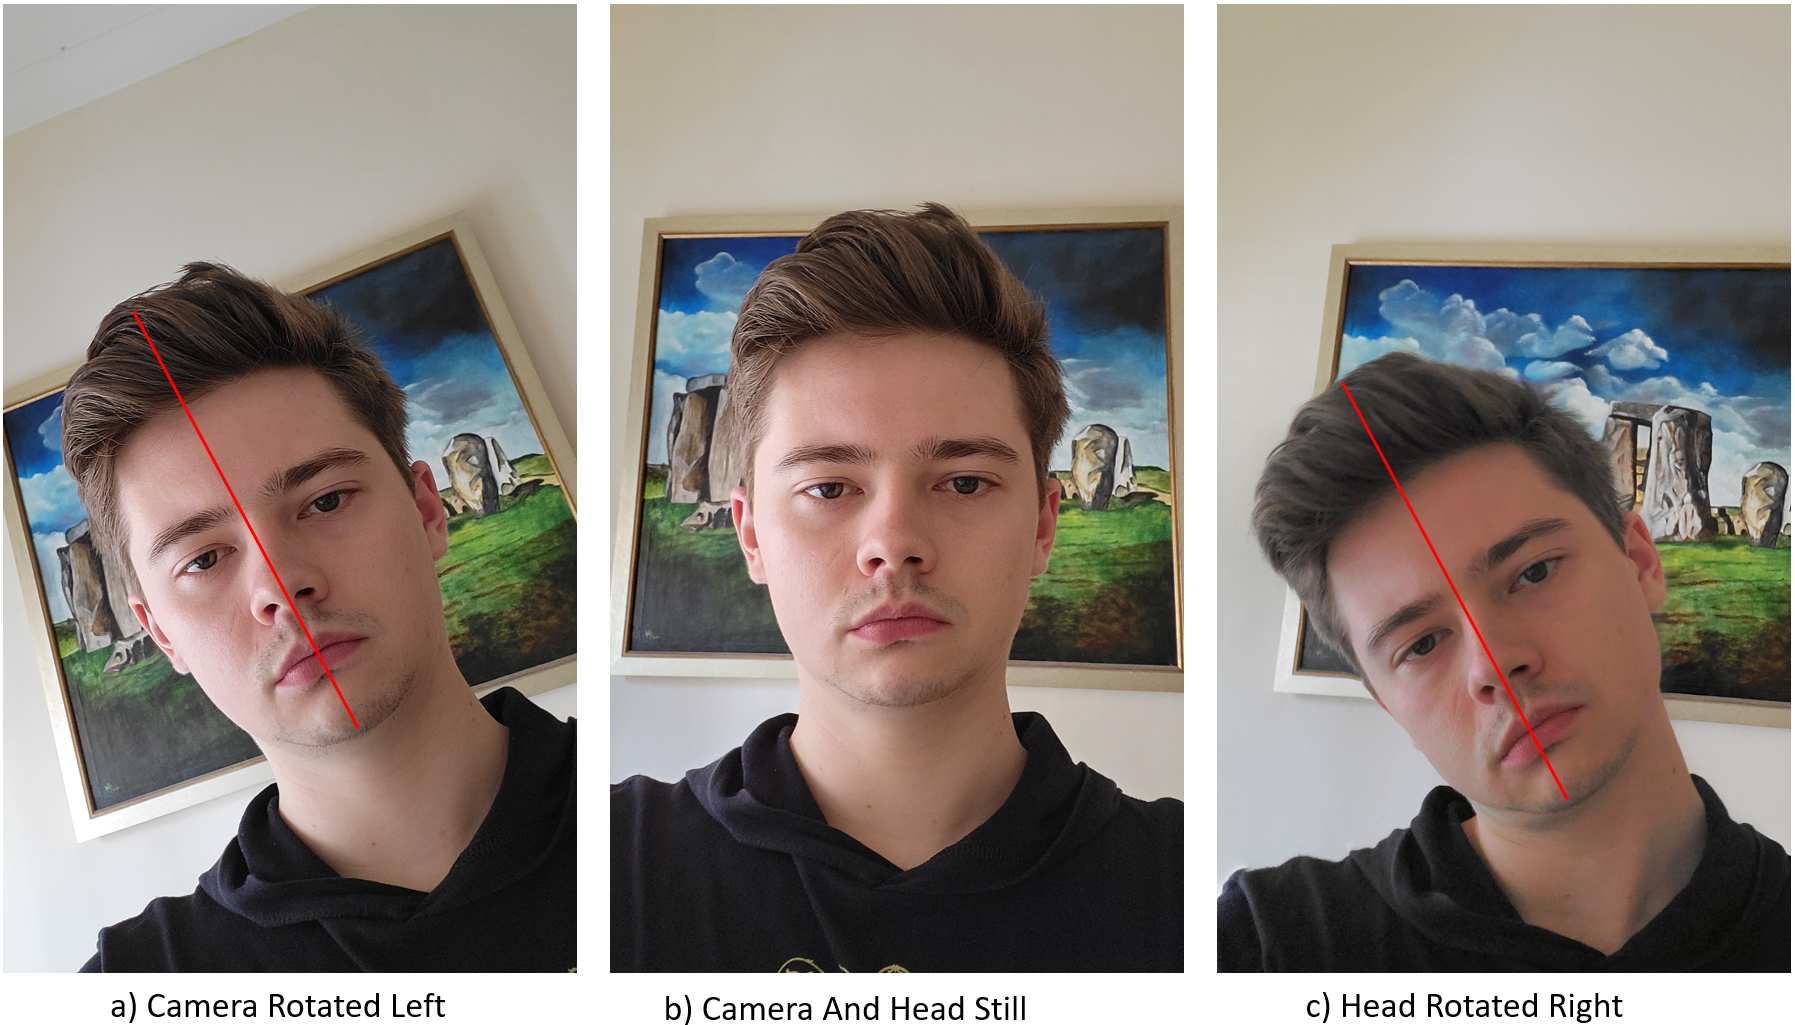
\includegraphics[width=0.65\textwidth]{figures/HeadOrientations.png}
  \caption{Demonstration of how changes in head or phone orientation can result in the same head orientation being observed by a smartphone's front-facing camera}
  \label{fig:teaser}
  \Description{Diagram showing how a the head pose observed by the front-facing camera of a mobile device, caused by the movement of the head, can be replicated by keeping the head still and instead moving the camera.}
\end{teaserfigure}

\maketitle
%% Content Lists %%

% \clearpage
% \restoregeometry
% \newpage

% \setcounter{page}{0}
% \pagenumbering{roman}
% \pagestyle{fancy}

% \tableofcontents
% \clearpage
% \newpage
% \addcontentsline{toc}{section}{\listfigurename}
% \listoffigures
% \clearpage
% \newpage
% \addcontentsline{toc}{section}{\listtablename}
% \listoftables
% \clearpage
% \newpage

% Tell TexCount to start counting words again
%TC:endignore

% Reset Page Styling and numbering for rest of doc
% \setcounter{page}{1}
% \pagenumbering{arabic}

    \section{Introduction}\label{sec:intro} % 0.5 Pages
%% What 
% State of The World:
Touchscreens have been the primary interface with which users interact with modern smartphones, either through directly touching UI elements (such as buttons or an on-screen keyboard) or through the use of touch-gestures. 
Over recent years there has been a trend of smartphone touchscreens increasing in size~\cite{xuesheng2018research}, which does not afford optimal reachability of the full screen for the thumb for interactions~\cite{le2018fingers}. This reduces usability for one-handed interaction, which is a common mode of use~\cite{hoober2013users}.
\\\\
An emerging solution to this is to include head gestures as an additional mode of input, by tracking the head via the smartphone's front-facing camera~\cite{gorodnichy2004nouse, deepateep2020facial, voelker2020headreach, roig2015face, hansen2006use, francone2011using}.
A problem with tracking something via a camera that can have a moving Point-of-View (PoV) is that changing the camera's PoV can \textit{look} like movement of the object being tracked.
For example, the user moving their phone to the left, will be treated the same as the user moving their head to the right, since the positioning and movement of the head from the front-facing camera's point of view will look the same, see \autoref{fig:teaser}.
Some papers knew of this issue and accept it as a feature~\cite{hansen2006use}, others note it as a known fault to be aware of~\cite{francone2011using, varona2008hands}, while others don't indicate whether this has been accounted for~\cite{gorodnichy2004nouse, deepateep2020facial, voelker2020headreach,roig2015face}.
\\\\
% Research Question:
In this paper we look to propose a system that can distinguish between the head or smartphone being moved. In being able to differentiate the two, it should also be able to recognise gestures based on the smartphone movement.

% Solution/What We Did:
In order to develop a proof-of-concept, a data driven approach was taken.
As such a study was performed to collect data: image sequences from the front-facing camera of the smartphone, IMU data from the smartphone, and 3D positioning of the user's head and the smart device via a motion capture system (to provide a ground truth).

With the motion capture data being synced to the IMU data and images, a system could be trained to recognise several gestures and learn to distinguish between whether an observed gesture was due to the smartphone or the user's head moving.

\tempnote{Pending confirmation of system's performance (what was actually delivered/produced) and how it could be extended upon.}
% What was the system's performance? Did we succeed?
% How is the work to be extended?

    % TODO: Do we need summaries after each subsection?
\section{Literature Review} % 2-3 Pages
In this section we will review existing literature to build an understanding of: the gestures we can expect to process, how they may be used and what they mean; Methods with which to obtain data pertaining to the pose of a head; and finally the means with which we can track movement and determine the gesture being performed.
% Types of Head Gestures (Pointing (Dietic & Manipulative) vs Semaphoric)
%   Since used by the systems mentioned in the intro, discuss these 3 types
%   Why would these types of gestures be used, what roles did they serve.
%   Examples of these gestures (with regards to systems referenced in intro)
% Probably a small section

% Head Tracking (From Smartphones)
% How track head, (Front facing camera, )
% Cascades, need face first, or one model (if using NN/ML solutions)
%   - IMU (From Head Mounted Displays and Head Mounted IMU)
%       - Will intend to use earbuds to collect IMU data of head, make footnote mentioning that this this was unfortunately not completed within this paper
%   - CNNs
%   - HAAR
%   - Alternatives (Feature extraction via histograms, etc)

% Head Gesture Recognition
% How did reviewed systems do this?
% Given data, how determine gesture performed, e.g. Dietic pointing (use raw data, e.g. calculate screen region/pointer position from data) vs Semaphoric/Manipulative classifying (given data, determine gesture performed)
%   - Derived
%   - Regression NN?
%   - RNN/LSTM (papers not specific to mobile phones)
%       - given a sequence, what class does it belong to?
%   - Markov Chain
%       - Given current state and new input, what is the new state?

% Merge last 2 sections into one?

\subsection{Gesture Classifications and Usage} % Types of Head Gesture
% Types of Head Gestures (Pointing (Dietic & Manipulative) vs Semaphoric)
%   Since used by the systems mentioned in the intro, discuss these 3 types
%   Why would these types of gestures be used, what roles did they serve.
%   Examples of these gestures (with regards to systems referenced in intro)
% Probably a small section

% Gesture classes and then discuss their examples / use-cases?
% Or
% Papers and examples, and then classification?

% Discuss why might want head gestures ?
%   - Any cases where these motions may be useful for SIIDs (Situationally Induced Impairments or Disabilities)?
% add more input options, not rely on using intuitive gestures that have since become system gestures (android navigation gestures) ~\cite{hueber2020headbang}

% Outline the types of gesture, and of those, which ones head gestures can b classified as.
% From example papers regarding head gesture control for mobile devices, look into 

Given our goal is to develop a means to distinguish head and phone gestures on smartphone devices, we first need to understand the gesture's we want to recognise and distinguish.
Here we will look at existing literature that outline the head and phone gestures you would expect to use while interfacing with a smartphone.

% Mention classes defined > mention ignore 2 as unrelated to head-gestures > explain exemplars of each type > Summary suggesting multiple employed by each system?
% Mention classes defined and list > mention ignore 2 as unrelated to head-gestures > describe several exemplars and what style/s they fit into?
% Mention classes defined and list > mention ignore 2 as unrelated to head-gestures > describe how in our review of literature that we classify as pointing/cursor manipulation vs semaphoric (gesture maps to action)
%
% https://eprints.soton.ac.uk/261149/1/GestureTaxonomyJuly21.pdf
% Breakdown the relevant gestures
After a review of gestures utilised within Human Computer Interaction literature \citeauthor{karam2005taxonomy} define five distinct classes with which we can differentiate between types of gestures utilised by the systems proposed in the literature~\cite{karam2005taxonomy}:
\begin{description}
    \item[Deictic] Gestures that involve pointing, and mapping this to either a specific object or location within the interface.
    \item[Manipulative] A gesture which indicates intent to manipulate some object.
    \item[Semaphoric] Gestures which map to a specific action or intent.
    \item[Gesticulative] Typically accompany speech, but not required to transfer meaning.
    \item[Language] A substitute to written or verbal language.
\end{description}

In our review of head/phone gesture systems we found that none utilised the Language or Gesticulative gesture styles, which is to be expected as we were focusing on gestures for control and interaction rather than for communication.
Of the 3 remaining gesture styles, we noted that systems rarely utilised a single gesture style. Either due to the gestures themselves being viewable as multiple gesture styles, being both semaphoric and manipulative, or by actively including different styles of gestures, such as pointing to a region, then using a sempahoric gesture to trigger an action.
% detail examples showing the gestures they decided upon, and why.
% example the types of gestures
% how might a phone gesture differ from head
% why might they look the same?
% yan2018headgesture, they explored existing head gestures (maybe focusing on those trackable via IMU over other methods?). Their study resulted in details shown in figure

\begin{figure}
    \centering
    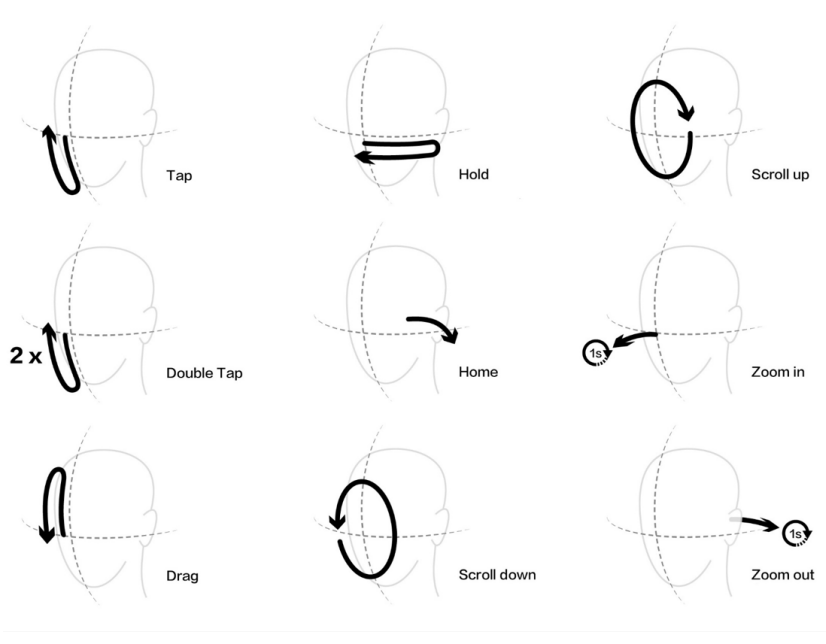
\includegraphics[width=0.5\textwidth]{figures/yan2018headgesture_fig2_proposed_gestures.png}
    \caption{\label{fig:yan2018headgesture_proposed_gestures} Proposed head gestures and their corresponding actions~\cite{yan2018headgesture}.}
    \Description[9 diagrams depicting the gestures proposed by \citeauthor{yan2018headgesture}]{9 diagrams depicitng the path of the nose taken to perform each gesture proposed by \citeauthor{yan2018headgesture}.} % TODO: Expand on this
\end{figure}

% \begin{figure*}
%     \centering
%     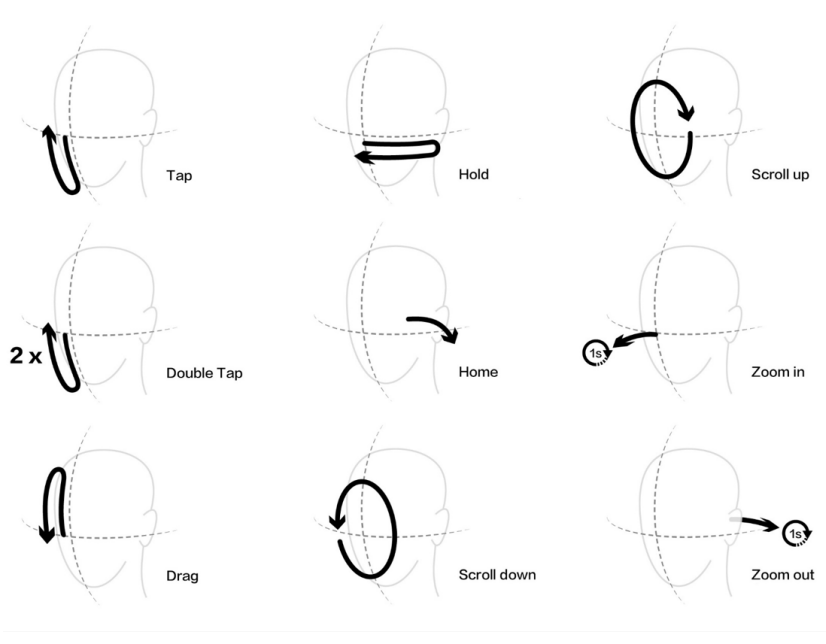
\includegraphics[width=\textwidth]{figures/yan2018headgesture_fig2_proposed_gestures.png}
%     \caption{\label{fig:yan2018headgesture_proposed_gestures} Proposed head gestures and their corresponding actions~\cite{yan2018headgesture}.}
%     \Description[9 diagrams depicting the gestures proposed by \citeauthor{yan2018headgesture}]{9 diagrams depicitng the path of the nose taken to perform each gesture proposed by \citeauthor{yan2018headgesture}.} % TODO: Expand on this
% \end{figure*}


An example of this can be seen in the work of \citeauthor{yan2018headgesture}~\cite{yan2018headgesture} who propose nine head gestures (\autoref{fig:yan2018headgesture_proposed_gestures}), the majority of which are purely Semaphoric, however several (such as scrolling, dragging, and zooming) could also be seen as Manipulative through the mapped action physically moving the content on screen.
\citeauthor{yan2018headgesture} derived these gestures through a study wherein participants where asked to proposed a set of head gestures, without being given an associated action. These gestures were then collated manually into a set of 80 gestures, which were then effectively voted upon by the participants for their respective actions.
The gestures with the most votes for a given action were selected, with some minor adjustments to ensure there were no clashes between actions.

Another system that utilised multiple gestures was EyeMu~\cite{kong2021eyemu}, which outlines several gestures that are performed by physically moving the smartphone, to improve user interaction when the user is forced to interact with phone single handed.
As with \citeauthor{yan2018headgesture}'s gestures, most are Semaphoric, but can be viewed as manipulative.
Some map to actual actions, e.g. flicking between items, others are less derivative and have less of a connection to the desired effect, e.g. moving phone closer/further from face to select an item / open a page.

% NOUSE
Two systems that were purely Deictic are Nouse~\cite{gorodnichy2004nouse} and a system developed by \citeauthor{varona2008hands}~\cite{varona2008hands}, both of which map the position of the user's nose, within images from the front-facing camera, to a location on the screen.
Neither system recognises sequences of motions of the head as gestures, other than recognising blinking and winking, which were recognised as an action to select what was under the cursor. 
You could also argue that these systems are also manipulative given they show a cursor and as such the head gestures are in an attempt to move the cursor to the relevant location.

% https://projet.liris.cnrs.fr/imagine/pub/proceedings/CVPR2012/data/papers/workshops/W01_05.pdf
One system which could be said to combine all three gesture styles would be the virtual 3D display proposed by \citeauthor{lopez2012head}~\cite{lopez2012head}.
Their system treats the smartphone screen as a window into a 3D box, visualised in \autoref{fig:lopez2012head_virtual_box}, where the region of the interior rendered is controlled via the user adjusting the position of their head with respect to the screen.
\begin{figure}
    \centering
    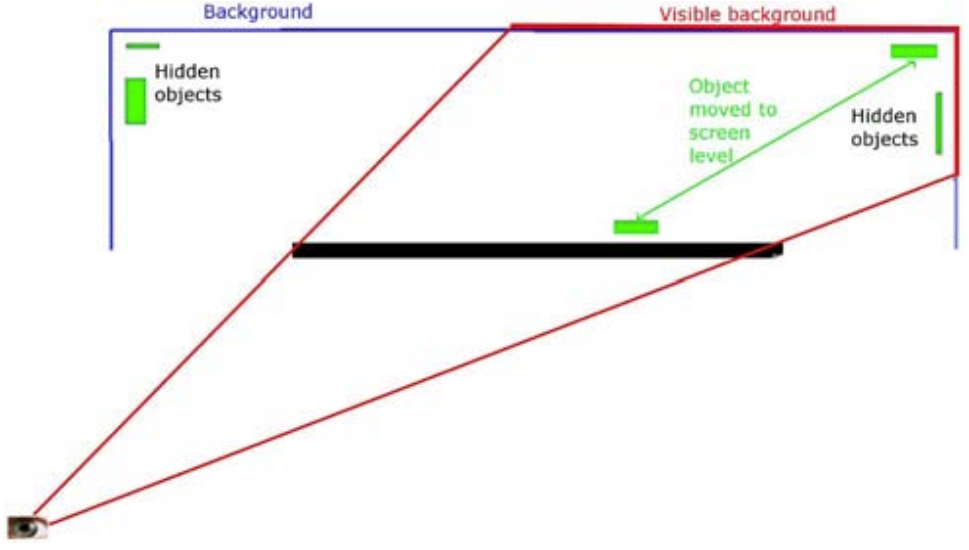
\includegraphics[width=0.45\textwidth]{figures/lopex_etal_virtual_box.png}
    \caption{\label{fig:lopez2012head_virtual_box}How user's perspective alters content that is rendered~\cite{lopez2012head}.}
    \Description{Diagram showing how a user's perspective alters content that is rendered in the app proposed by \citeauthor{lopez2012head}.} % TODO: Expand on this
\end{figure}
The tracking of relative positioning of the head to adjust the perspective of what is rendered can be seen as a form of both Deictic and Manipulative gesturing, as the user is looking at different regions within the interior of the virtual box by simply changing where they are looking, but with the intent to adjust the visible interior of the virtual box.
The system also provides Semaphoric gestures when interacting with specific programs; in one example they use a browser, with which they can look to the edge of the page to reveal the bookmarks bar.

% What conclusions can we make from this? 
% The types of gestures we expect (pointing, both manipulative and deictic, and semaphoric)

% Head bang and reach
% Initially used to 

% Phone gestures
% https://dl.acm.org/doi/pdf/10.1145/3462244.3479938

\subsection{Head Localisation}
% Image processing using front-facing camera
%   CNN (extract face position or pose/features)
%   HAAR Cascades (extract face position, or extended to features)
%   HSV Image Segmentation (extract face position, additional processing for pose etc)
%   Optical Flow (maybe extract face, or just use Optical flow to guess movement, might not need this one)
% IMU hardware (cap mounted IMU or headset)
%   Headset (not applicable)
%   Bespoke accessory with IMU, maybe use earbuds with IMU
% LIDAR/Depth Cameras (if time/space, if not, mention off-hand ignoring as not available on all devices, and not something you could buy after the fact, like headset or earbuds)
Before being able to distinguish between head and phone gestures, we first need to extract them. 
To start with we will be reviewing the methods in surrounding literature to extract relevant data required to track head gestures through the use of a smartphone.

The naive approach often taken for finding a face, or more generally a person, within an image is to perform colour segmentation~\cite{huang2004robust,bin2007rgb,chan2004face}, which involves taking an image and filtering the pixels based on a range of colour values that have been chosen as representing skin-tones.

While simple, and given favourable conditions, effective, this approach has several drawbacks:
\begin{enumerate}
    \item Detection of objects which have colours that have similar colour and chrominance levels, as noted by\citeauthor{bin2007rgb}~\cite{bin2007rgb}.
    \item Determining the values with which to segment the image, i.e. what colours will we accept as skin-tone? During their system evaluation \citeauthor{chan2004face}~\cite{chan2004face} used participants with similar skin-tones to improve the system's robustness.
    \item Dependence on environment lighting.\\
        All three of the papers above~\cite{huang2004robust,bin2007rgb,chan2004face} do make use of the HSV/yCbCr colour spaces, which make them more robust to changes in lighting intensity, however these systems can still be susceptible to changes in lighting temperature, colour, or shadows.
\end{enumerate}\nl
% \subsubsection{HAAR Cascades / The Viola Jones Algorithm}\nl
A less naive approach is the Viola-Jones algorithm proposed in 2004~\cite{viola2004robust}, used in digital cameras, smartphone camera apps, and several head gesture systems~\cite{kim2017real, neto2012real, francone2011using}.
Rather than looking for skin-tone to find faces, it uses the difference of intensity between regions of pixels, and checks if they match a set of templates, Haar-features. These features compare the relative intensity of 2, 3, or 4 neighbouring regions, e.g. is the centre of a region brighter than the regions to the left and right. 
The algorithm proposed by \citeauthor{viola2004robust} uses a degrading cascading classifier\footnote{Where a traditional cascading classifier will have possibly have 2 branches at each node, a degrading one will always exit, returning nothing, on one of the branches of each node.} to apply these Haar-features on an integral image\footnote{A representation of the input image that permits an efficient means to calculate the sum of a rectangular region of the image with just the for corner points.} and will return a bounding box for each face found.

\citeauthor{kim2017real} build upon the Viola-Jones algorithm, still utilising Haar features but building their classifier to return the locations of four facial features: left eye, right eye, nose-tip, and mouth, in place of bounding boxes~\cite{kim2017real}.

A more typical approach however is to use the Viola-Jones algorithm to retrieve the bounding box of faces within the image, and then perform further processing to extract facial features~\cite{neto2012real, francone2011using, kim2017real}.
% ~\cite{neto2012real} Also utilise HAAR-like features in a classifier, however they simply use this to identify the region of the image that contains a face, and then utilise a histogram of pixel intensity (amount of variation in a given slice of the image) to identify the eyes.
% This is done once during calibration to then extract the eyes (left eye 30\% along the line, right is 70\%) and nose (if the eyes are $d$ far apart, the nose is $d*0.45$ below the midpoint between the eyes), assuming head is upright and user is facing camera.
One downside with the algorithm that \citeauthor{viola2004robust} note is that it cannot reliably detect faces that are rotated ±15\textdegree, while the person is still facing the camera, or ±45\textdegree, where the person is facing off to the side of the camera.
% An aside on use to extract location of face, but no features
% Application of filters representing features found on common faces.
% Applied in a cascade, e.g. only check for next set of features if found large one.
% Used to reduce search space / and limit data that needs processing.

Another solution present in the literature, that is invariant to face pose, is the use of depth cameras. 
In particular we found the use of Apple's ARKit framework used alongside the front-facing depth camera (on supported iOS devices)~\cite{voelker2020headreach,hueber2020headbang,deepateep2020facial}.
ARKit provides a reliable 3D representation/positioning of the face and its features  which could be used for tracking the head's movement.
The only downside of this approach seems to be the requirement of the hardware and OS in order to use the ARKit framework.

The final solution we reviewed was the use of Convolutional Neural Networks (CNNs).
YuNet~\cite{yu2022yunet} for example outputs the bounding box along with the positions of the eyes, nose tip, and the corners of the mouth. YuNet is in fact the replacement suggested by OpenCV for detecting faces, which previously used and recommended the Viola-Jones algorithm.

\citeauthor{yan2021fast} propose a CNN which instead predicts the roll, pitch, and yaw of a face provided within an input image~\cite{yan2021fast}. With their CNN they were able to observe reduced error in their predictions compared to existing tools.

The benefit of a CNN is that they should be invariant of head rotation, given the training data includes samples of heads at different rotations.
A potential downside is the need for sufficient processing power. However there do now exist mobile variants of popular Neural Network frameworks, such as TensorFlow, with TFLite, and PyTorch, with PyTorch Mobile, which make running CNNs feasible on mobile devices.

% Android MLkit for face detection?

% Some use HAAR cascades to narrow down region
% Some alo output similar to HAAR, e.g. bounding box

\subsection{Phone Localisation}
% We now have several methods we can refer to in order to determine the head gesture being performed by a user, however we now need to explore the final area in the related works: recognising phone gestures. 
During our review of related works we came across several means of localising a smartphone / tracking a smartphone's movement, each with varying degrees of feasibility.

The least reasonable methods do not bare reviewing due to unrealistic expectations of the population of smartphone users, such as the need for a Motion Capture (MoCap) system~\cite{buschel2017investigating} or the use of a Head Mounted Display with a mounted tracking marker~\cite{mohr2019trackcap}.
These may be suitable in specific environments, but are not reasonable in meeting our goal.

A more reasonable set of methods involve localising the smartphone's position relative to its environment.
\begin{figure}
    \centering
    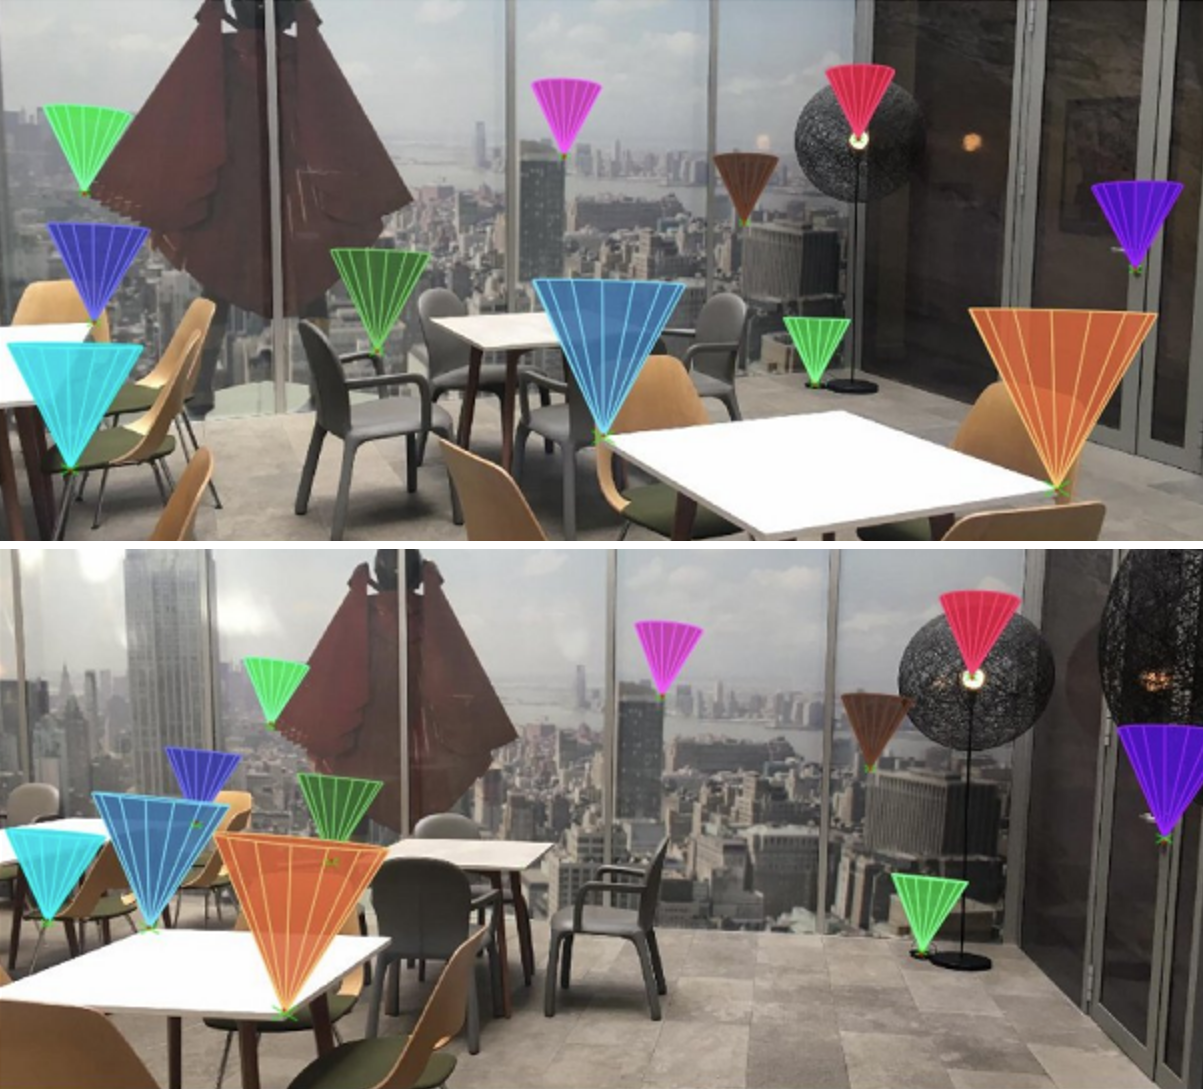
\includegraphics[width=0.45\textwidth]{figures/CameraTracking.png}
    \caption{\label{fig:barber2016camera_camera_tracking}Figure showing points being tracked~\cite{barber2016camera}.}
    \Description{Figure showing points being tracked.} % TODO: Expand on this
\end{figure}
One method is 'camera tracking', wherein the movement of the camera is estimated through analysis of an image stream from the rear-facing camera. This is a technique common-place in VFX to recreate the path taken by a camera in 3D~\cite{barber2016camera}, \autoref{fig:barber2016camera_camera_tracking} shows extracted 3D movement being used to track 3D cones into a video. However this technique has also been extended for use in Augmented Reality applications~\cite{jiang2000camera}.
Unfortunately this isn't reasonable to use on current modern mobile phones as they don't all support the ability to capture images from multiple cameras (some via software, others due to hardware limitations). As such we will not be able to utilise the rear camera as the front-camera will be required to track the user's face in our proposed system.

Another solution is the use of either Depth-Cameras or LiDaR and tracking the smartphone's movement through the observed 3D space.
Unfortunately these require special hardware that isn't available on most smartphones; most depth cameras that exist on modern smartphones are front-facing and the only current mainstream phones to provide a LiDaR on the rear of the phone are the iPhone 12 and 13 Pro series.

The only method we found to be reasonable and feasible was to record the linear and angular acceleration of a smartphone's Inertial Measurement Unit (IMU)~\cite{mantyla2000hand, kratz2013combining, neelasagar2015real, garcia2014contextualized}. 
An IMU provides the acceleration experienced in the 6 Degrees of Freedom (DoF)\footnote{3 Linear Axis: X, Y, Z, 3 Angular Axis: Yaw, Pitch, Roll} the smartphone can be manoeuvred through.
A common issue however with processing IMU output is noise, as noted by \citeauthor{neelasagar2015real}. To address potential noise they utilised low and high pass filters on the acceleration data. 

\subsection{Gesture Recognition}
% Head Gesture Recognition
% How did reviewed systems do this?
% Given data, how determine gesture performed, e.g. Dietic pointing (use raw data, e.g. calculate screen region/pointer position from data) vs Semaphoric/Manipulative classifying (given data, determine gesture performed)
%   - Derived
%   - Regression NN?
%   - RNN/LSTM (papers not specific to mobile phones)
%       - given a sequence, what class does it belong to?
%   - Markov Chain
%       - Given current state and new input, what is the new state?
Knowing how we can obtain facial features and the 'pose' of the user's head through a front-facing camera, and the localisation of the smartphone itself, the next step is to be able to recognise gestures performed by the user with either their head or the smartphone.

% \subsubsection{Relative Positioning}\nl
% NN vs Function, how best to phrase?
% Used for Pointing (Dietic)
% Great if data in is accurate (IMU may not be ideal without filtering)
One solution employed by papers proposing systems that tracked Deictic pointing gestures (and possibly Manipulative pointing gestures), was to simply use the raw data, or a function of the data, to map detected facial features to a location within the UI.

A common approach was to take the position of the nose and map it to a point on the screen. This could either be used to manipulate a cursor~\cite{gorodnichy2004nouse, varona2008hands, onuki2016combined}, allowing the user to move their head to highlight specific places on the screen, or to highlight the region of the phone the user is looking~\cite{hueber2020headbang,voelker2020headreach,roig2015face}.
% \subsubsection{Recurrent Neural Network (RNN)}\nl
% Write out the 
% Given a sequence, classify the type of motion
% not ideal if don't have known fixed number of frames, unless staggered

For semaphoric gestures you need to be able to be able to identify the gesture within a sequence of input.
An RNN is a Neural Network that takes a sequence of elements and has an internal state that is updated by some function of the current element being processed and the current state.
\citeauthor{sharma2018recognizing} proposed the use of an RNN in order to recognise head gestures, wherein the RNN input was a sequence of facial landmarks extracted from a sequence of images~\cite{sharma2018recognizing}. 
An advantage of using an RNN is that you don't strictly need to know exactly when the in the sequence the gesture was performed, just that it is present within the sequence.
A downside however is that internal state isn't maintained between predictions, as such you \textit{must} provide a sequence and the input sequence \textit{must} always be of a fixed length\footnote{This is to the best of our knowledge using common neural network frameworks such as TensorFlow and PyTorch}. Input must there for be broken-up to fixed lengths, either requiring padding prior to/after the gesture recorded (if you do not have enough elements for the required sequence). To break-up the input you need to either run the model each time-step, providing a rolling window representing the last $x$ frames of state, or to have another means to segment your recorded input to then pass into the RNN.

% \subsubsection{Hidden Markov Model (HMM)}\nl
% Given current state and new input, determine the new state
% Great if continuous input
% Another way that a Semaphoric gesture can be described is via a set of possible states, e.g. head poses or movement, and a set of rules which describe how these states can change.
Another method for predicting Semaphoric gestures from a sequence, is to use Hidden Markov Models (HMMs)~\cite{elmezain2008hidden, terven2014robust}.
A HMM describes the possible hidden states a system can be in, the probabilities/rules for transitioning from one state to another, the sates that can be observed, and the probability that a given observation arises from each hidden state.
For example, the HMM employed by \citeauthor{elmezain2008hidden}~\cite{elmezain2008hidden} has the gestures as its hidden states, in this case arabic numbers, with the possible observations being a quantised direction\footnote{To reduce the possible observation space, the angles from 0\textdegree to 360\textdegree are bucketed into a range of 0 to 18} that the user's hand travelled, captured via a camera. The probabilities of the sequence of observations would be observed for a given number drawn by the user can then be trained.

% Maybe some reinforcement learning stuff?

    \section{Data Collection} % < 1.5 Pages

% Outlines:
% - What gestures we want to recognise, based on papers from lit review (maybe own small section?)
% - Taking a data driven approach, what data will we collect

% Distinguishing Between Head and Phone Movement (Methodology)
%   Redefine goals of the system/research objectives
%   Rough outline of the technology we aim to use?
%   Outline data we need

This section details the process undertaken to develop the system which can meet the goal (outlined in \autoref{sec:intro}): distinguishing between head and phone based gestures on a smartphone.

% \subsection{Data Collection Study} % < 1.5 Pages
% outline
% - Taking data driven approach (intro to section)
% - The data we'll be collecting

In order to develop the aforementioned system we opted to take a data-driven approach.
%  The benefit of taking a data-driven approach is that we can leverage Machine Learning, and train the system with exemplar data, rather than needing to manually determine the features and derive the algorithm needed to accomplish our goal.

For a data-driven approach to work we need to first determine what data we need to collect in order to train our system. We have identified the following types of data:
\begin{description}
    \item[Images From The Front Facing Camera]\nl 
    Though a depth camera would likely be more reliable and accurate in extracting the shape/pose of the user's face, it does require hardware that is not yet standard on all smartphones. To enable our system to be run on as many smartphones as possible we will be opting to detect and track the user's head via the front-facing camera, for which we found many techniques from which to extract the user's head movement~\cite{varona2008hands, lopez2012head, viola2004robust, kim2017real, neto2012real, francone2011using, yan2021fast}.
    \item[Smartphone IMU Data]\nl 
        To understand whether the smartphone's PoV is changing we need to know how it is moving. 
        As noted in our review of surrounding literature, the most feasible means to do this is with the IMU present in modern smartphones~\cite{mantyla2000hand, kratz2013combining, neelasagar2015real, garcia2014contextualized}, which will allow us to track the phone's linear and angular acceleration.
    % \item[Head Acceleration Data]\nl 
    %     If we can determine the movement of the smartphone via acceleration data, it is reasonable to see if we can also do the same with the user's head.
    \item[Ground-Truth Data]\nl 
        In order to accurately train a model that can achieve our goal, we will need some Ground-Truth data. This will include the gesture the data is associated with, so that the system can classify gestures. It will also be helpful to capture the actual head and phone poses/motion during given gestures such that we can aim to train a model that can predict the movement of the head and phone.
\end{description}

% - The tools and apparatus we'll be using
% - The data collection app (how it works, issues, output format)
% - Gestures we chose to collect (based on lit review systems, (only subset of pointing, only looking at 8 points around the screen, rather than anywhere))
\subsection{Apparatus and Techniques}

\subsubsection{Pixel 4a}\nl
To collect images and IMU data we opted to use a Pixel 4a smartphone.
The operating system is Android 12, and the phone's dimensions are 144mm x 69mm x 8, with a screen size of 5.6 inches.
This was chosen as it we believe it to be fairly representative of modern smartphones (at least for the android market share), with reasonable dimensions that should not be too difficult to hold for our participants, a front-facing camera capable taking up to 1080p resolution images, an IMU, and a sufficiently powerful processor such that we should not need to worry about an application that can record photos and capture IMU data stuttering and missing data.

\subsubsection{Data Collection Application}\nl
\begin{figure*}
    \centering
    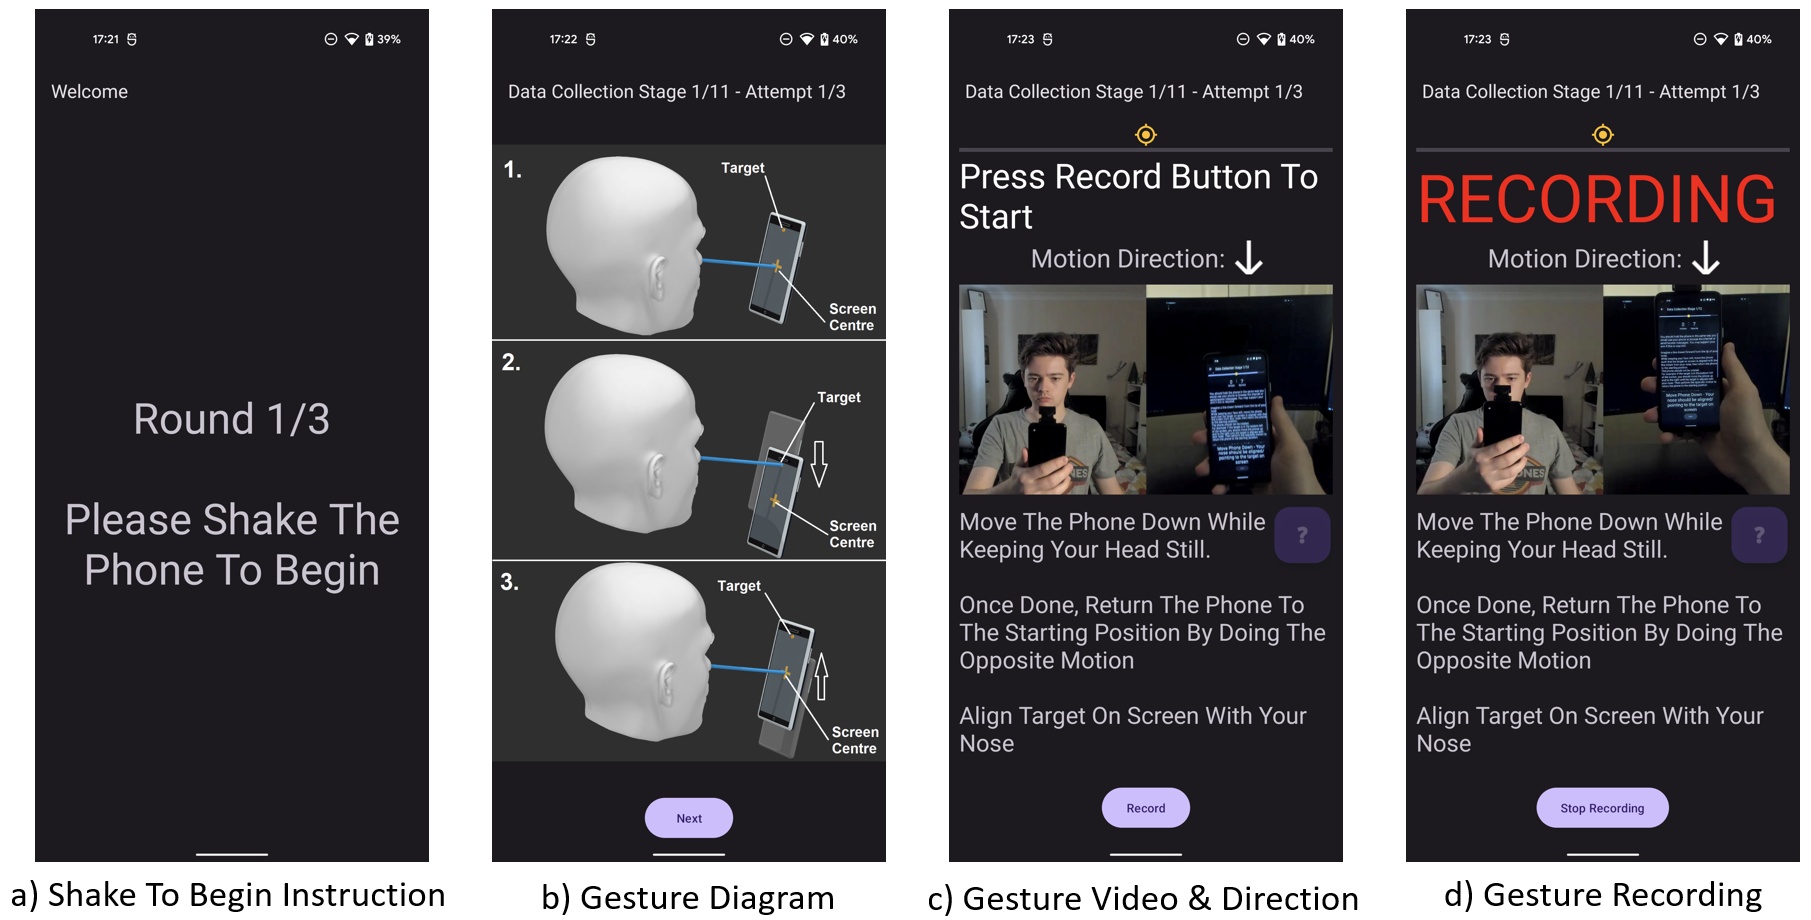
\includegraphics[width=\textwidth]{figures/DataCollectionApp.png}
    \caption{\label{fig:data_collection_app} Various stages of the data collection app UI}
    \Description{Figure showing 4 stills taken from our data collection app. A: Instructions asking participant to shake the phone to start. B: Diagram showing how to perform upcomming gesture. C: Video showing how to perform current gesture, with POV from phone camera and user POV, along with additional symbolic and textual direction cues. D: Application informing participant that data is being recorded.}
\end{figure*}
% Discuss how the application will collect data (images and need to save as raw yuv bytes, IMU with $50Hz$ sample rate saved to csv)
% How data will be organised
% How app will provide instructions
% Shake detection for synchronising with ground-truth data
Since the Pixel 4a runs on Android, we opted to develop our data collection app using Kotlin and the Android framework.

The application was designed to instruct the participants on how to perform a series of gestures and to provide the ability to record data from the IMU and images from the front-facing camera as participants performed the gestures.
To instruct the participants on how to perform the gestures, we included three different mediums for describing the gesture: Text, Images, and Video.
Before a participant could record a gesture, they would first be shown a diagram that outlines what they should be looking at on the screen, and how the head or phone should be moved. This would be accompanied by some text that would describe the same motion in more detail, in order to try and resolve any confusion with the participant's understanding of the diagram.
Once the participant has observed the diagram and text, they are then shown a video containing the viewpoint of both the phone and the head during the gesture. This is accompanied with a symbol indicating the direction the phone or head should be moved or turned, and a further textual description of the direction the phone or head should be moved.
% We understand that having these many instructions could lead to too much information being provided to the participant, however we were balancing between having too much information, and ensuring the right medium of the information was available to the participant.

To begin recording the gesture shown, the participant presses a record button, placed at the bottom of the screen to be easily reached with their thumb. At this stage the record button will be frozen, to prevent the recording be cancelled prematurely from a double tap, and the application will begin recording images and IMU data for a minimum of 2 seconds. After the 2 seconds have elapsed, the record button is unfrozen and the participant can chose to stop the gesture recording if they have finished. If the recording is not stopped, the participant is given an additional 8 seconds to perform the gesture, after which the recording will be automatically stopped, and the next gesture shown to the user.
We employ a limit for the time to perform a given gesture as none of the gestures we intend to capture should take more than a few seconds to perform, however we did not want to risk cutting off a gesture mid-performance.
This is then repeated for each gesture we wish to capture and then each gesture is shown again 2 more times, such that each gesture should be performed 3 times. We include repeats of each gesture to include additional variance in the recorded data.

The recorded data for each gesture is saved into device storage, under a directory path starting with the participant id, followed by the gesture take number, then the gesture name, and finally the gesture direction. For example "\verb|4/attempt_0/ROTATE_HEAD/RIGHT|"

Requesting data from the IMU was a simple task, you simply need to register a \verb|SensorListener| for the type of data you want. In the interest of collecting as much data as possible, in order to give us more options with regards to which data to use for our model, we setup six listeners: three to retrieve the linear acceleration, and three to retrieve the angular acceleration.
The first linear acceleration sensor provides the acceleration along each axis ($X$, $Y$, and $Z$), but this includes gravity and any bias that may exist in the sensor, the second excludes the bias, and the third excludes bias and gravity.
The first angular acceleration sensor provides the acceleration about each axis (roll, pitch, and yaw), but may include bias, the second removes this bias, and the third provides a quaternion representing the phone's orientation with respect to magnetic north and gravity.

Unfortunately it was not possible to request all the data with a single listener. To ensure the IMU data recorded was synchronised, we had the listeners store the latest values in a set of arrays, and had a timer that would trigger at $50Hz$ to pull the latest values from the arrays and store them with the current timestamp in a csv for the current take, gesture, and gesture direction.

Capturing the images was a more difficult challenge.
The easiest option would be to record a video with a fixed frame-rate, however this would result in the captured frames of images being compressed, and in a format that would not achievable in deployment of the system we aim to propose, i.e. we would not intend to record and decode a video in realtime to capture images for head gesture recognition.
Instead we setup a repeating camera request with the front-facing camera, which when activated would try to retrieve an image from the camera image buffer as often as possible. This does come with 2 downsides however: 
\begin{enumerate}
    \item The capture rate is not fixed. This could be a positive, by providing variance to the data collected, but could reduce the learning rate of the system we aim to propose as it will also need to learn how to adapt to images that can occur inconsistently.
    \item The captures can be halted by Garbage Collection. Though this didn't seem to be an issue with the IMU data collection, we observed some deltas between images being taken jumping sporadically. We believe this to be down to GC events, as they appear within the profiler when the deltas spike.
\end{enumerate} 

Images were saved as raw YUV bytes, the image format provided by the camera, into an \verb|images| directory for the current gesture recording, with the timestamp at the time of capture being used as the file name.
We did originally try to convert the YUV image into RGB, which we would expect to feed into the system we will propose, however this required significant processing time and memory, resulting in a low sample rate and images still being converted and saved after the gesture recording had finished. If the participant was recording gestures at a reasonable rate this would result in an Out of Memory Error and crash the application.
We did try to utilise OpenCV for android, however we were unable to package it into the application such that the required native binaries were available at runtime.
By saving the raw YUV bytes we were able to leave the RGB conversion to be performed after the data was collected, and increased our sample rate for images. This does provide a bit of disparity between the collected data and the data we will require for the system we will propose, primarily the delta between samples, however this does allow use to treat the collected data as being taken from a smartphone with better hardware, which could achieve higher sample rates and conversion to RGB. We can also aggregate collected data to lower sample rates to be more realistic with what the Pixel 4a can achieve.
% The application was designed to show participants a motion (a gesture and direction/variation) to perform. This is detailed in text, images, and a video. \tempnote{Include figures to show this (spread accross columns at top of page?)}
% The participant would then be asked to perform this motion after pressing a record button. While recording the app would do the following:
% \begin{itemize}
%     \item Capture images as frequently as possible from the front-facing camera, saving them as raw YUV bytes, with the UTC timestamp as the name.
%     \item Record the smartphone IMU data (linear and angular accelerations), saving them to a csv with the UTC timestamp.
%     \item Record the earbud IMU data (linear and angular accelerations), saving them to a csv with the UTC timestamp.
% \end{itemize}
% % Link to class diagram, or do we just want photos?
% Once the participant has finished with the motion they could press the same button to stop the recording. Otherwise the recording will automatically terminate after 10 seconds, since the gestures shouldn't take more than a couple seconds to perform and the phone has limited RAM and storage with which to save data.
% To prevent accidentally stopping the recording too soon, say by accidentally double-tapping the screen, we disable the button for 2 seconds.
% Once a motion has been recorded, the app shows the participant the next motion to perform. When the participant completes the final motion to perform, the app returns to the first motion. This repeats two times, such that each motion is captured 3 times. This is to collect variance in each motion for each participant.

To allow us to synchronise the data collected from the smartphone and the ground-truth data we will also be collecting, we have the application ask the participant to shake the phone prior to beginning a round of gestures. For the shake to be recognised it must exceed a total magnitude of 2$g$. If a shake is detected as exceeding 2$g$ the current timestamp and the acceleration of the phone, taken from the IMU, are recorded to a csv. We can then hopefully find the shake in the ground-truth data to be able to line-them-up and generate a csv with both the data from the phone and the ground-truth.

\subsubsection{Motion Capture System}\nl
To track the actual positions of a participant's head and the smartphone, we will be using a the Motion Capture (MoCap) system managed by the CAMERA team on the University of Bath campus.

\nl\tempnote{Camera count and software}\\
To track both the head and the smartphone a set of ten markers, that can be tracked by the MoCap system, will be used (five markers each).
One marker will only allow you to track the location of an object. Two markers will allow you top derive the pitch and yaw of the object with just the use of some trigonometry and the vector defined by the two points. A third marker will allow you to also extract the yaw of the object using the same trigonometry, however the third point must be placed such that a right angled triangle is formed by connecting the points.
The additional 2 markers used are to allow us to distinguish which set of markers are associated with each object being tracked, being placed in unique positions around the three main points.

To affix the tracking markers to a participant's head we attach them onto a rigid square of foam, in order to prevent the relative positions of the markers to each other being distorted, and then attach this to a skull-cap that the participant can place upon their head.
The markers are attached to the skull-cap such that the markers should be at the rear and centre of the participant's head. 
We chose to track the rear of the head as having tracking markers present on a participant's face could result in the markers being picked-up in the images collected from the front-facing camera, which could impact the ability to detect faces or extract the participant's head pose.

A slight issue with affixing the markers with a skull-cap is that they won't always be in the same place with respect to the participant's face, due to everyone having slightly differently shaped faces. For example a person with a taller head will have the markers higher-up from the base of their neck, someone with a deeper face will have the markers further away from their nose.
We could take measurements of each participant's head and determine the exact relative position of the trackers to a set of facial landmarks, however we do not believe the this to be significant issue as the data will still allow us to track the relative movement of the head, which should be enough to train a model to recognise the gestures. This will also introduce a small amount of variance into the training data which should aid reducing the impact of over-fitting.

To affix the markers to the smartphone we 3D printed a mount that the phone could be snapped into and the markers attached.
To ensure the markers would not impact the participant's ability to hold and manipulate the phone one-handed, we had the mount extend from the top of the phone. To ensure the markers would be visible to the MoCap system through all the motions the smartphone would be moved through for the collection of gesture data, and to ensure the markers and mount would not be visible to the front facing camera, it was mounted at 22.6\textdegree away from the front of the phone.
Due to the mount being printed out of plastic, it was not particularly grippy, and as such only friction was preventing it from moving side-to-side on the phone. This should not be a significant issue, as with the participant's grip on the phone, it should not move significantly while performing gestures, and may only slip as a participant adjusts their grip. As with the markers for the head, this should still allow use to get the relative movement of the phone during the recording of gestures.
\nl\tempnote{Image of the 3D printed mount}

The output provided by the MoCap system was an fbx file which contains the positions of each of the markers, measured cm, captured at a sample rate of $60Hz$. 

% - Study Outline
%   - What participants would be asked to do
%   - Need footnote or aside to mention that originally intended to also capture IMU data from an eSense earbud, but was not ultimately collected, hence why earbud included in steps
\subsection{Procedure}
% grab instructions from PIS
Upon attending the study, the participant will be provided an information sheet which will provide details on the study, such as the purpose, what data will be collected and managed, what they will be asked to do. Once read they will read through and sign the consent form if they are happy to continue.

If consent is obtained, the participant will be asked to enter the Motion Capture stage (the space that is viewable to the MoCap system) and asked to wear the skull cap with the motion trackers attached.
The MoCap system will then begin recording. and the participant will be provided with the smartphone, which will already have the data collection app running, and asked to read through the disclaimer, which reiterates what data is captured. Once they have read the disclaimer, the participant will shake the smartphone to start with their first take of gestures.

Within the data collection app, the participant will be shown a diagram and text describing the gesture they need to perform. Once understood they are able to move on to show a video of the gesture, from both the phone's Point of View, and the participant's, along with additional brief text and a symbol describing the direction of motion for the gesture.
If the participant has any questions regarding the motion they need to perform, they were welcome to ask the researcher present to further explain the motion, or to provide a demonstration.
The participant will additionally be instructed to hold the phone as they typically would when using their smartphone, to say browse the internet or read messages.

Once the participant is ready to perform they gesture they will tap the record button and perform the gesture. The recording will then be stopped when they press the button again after completing the gesture, or it will automatically stop after 10 seconds.
The next gesture will then be shown to the participant.

This is repeated until the participant has completed each gesture three times. Between each round of gestures the participant will be asked to shake the smartphone before being shown the next round of gestures. Once all the gestures have been completed, the participant will remove the skull cap, hand-in the smartphone, and read-through a debrief sheet, containing an additional request for consent to use the data.

Regarding the gestures participants were asked to perform, we decided upon 11 gestures, each with 2-8 variations (effectively directions the gesture could be performed in), resulting in a total of 44 distinct motions to obtain samples of. A breakdown of the gestures and variations can be found under \autoref{app:gestures}.

\subsection{Participants}
\begin{table}
    \centering
    \caption{Breakdown of Participants}
    \label{tab:participant_breakdown}
    \begin{tabular}{ c | c | c }
        Participant ID & Age & Gender \\
        \hline
        0 & 23 & Female \\
        1 & 25 & Male \\
        2 & 21 & Female \\
        3 & 24 & Male \\
        4 & 26 & Male \\
        5 & 24 & Male \\
        6 & 27 & Male \\
        7 & 23 & Female \\
        \hline
    \end{tabular}
\end{table}
For our study we recruited 8 participants from the University of Bath campus who were between the ages of 23-27.
37.5\% of the participants identified as female, the remaining 62.5\% identified as male. A full breakdown can be see in \autoref{tab:participant_breakdown}.

% - The study data
%   - breakdown of participants
%   - Recordings captured (/motions)
%   - Data analysis (distance moved by gesture, time taken, face detected (using YuNet and OpenCV))
%       - Why might expect
%       - Issue accurately calculating rotation delta (maybe use this? https://forum.unity.com/threads/shortest-rotation-between-two-quaternions.812346/)
\subsection{Results}
\begin{figure*}
    \centering
    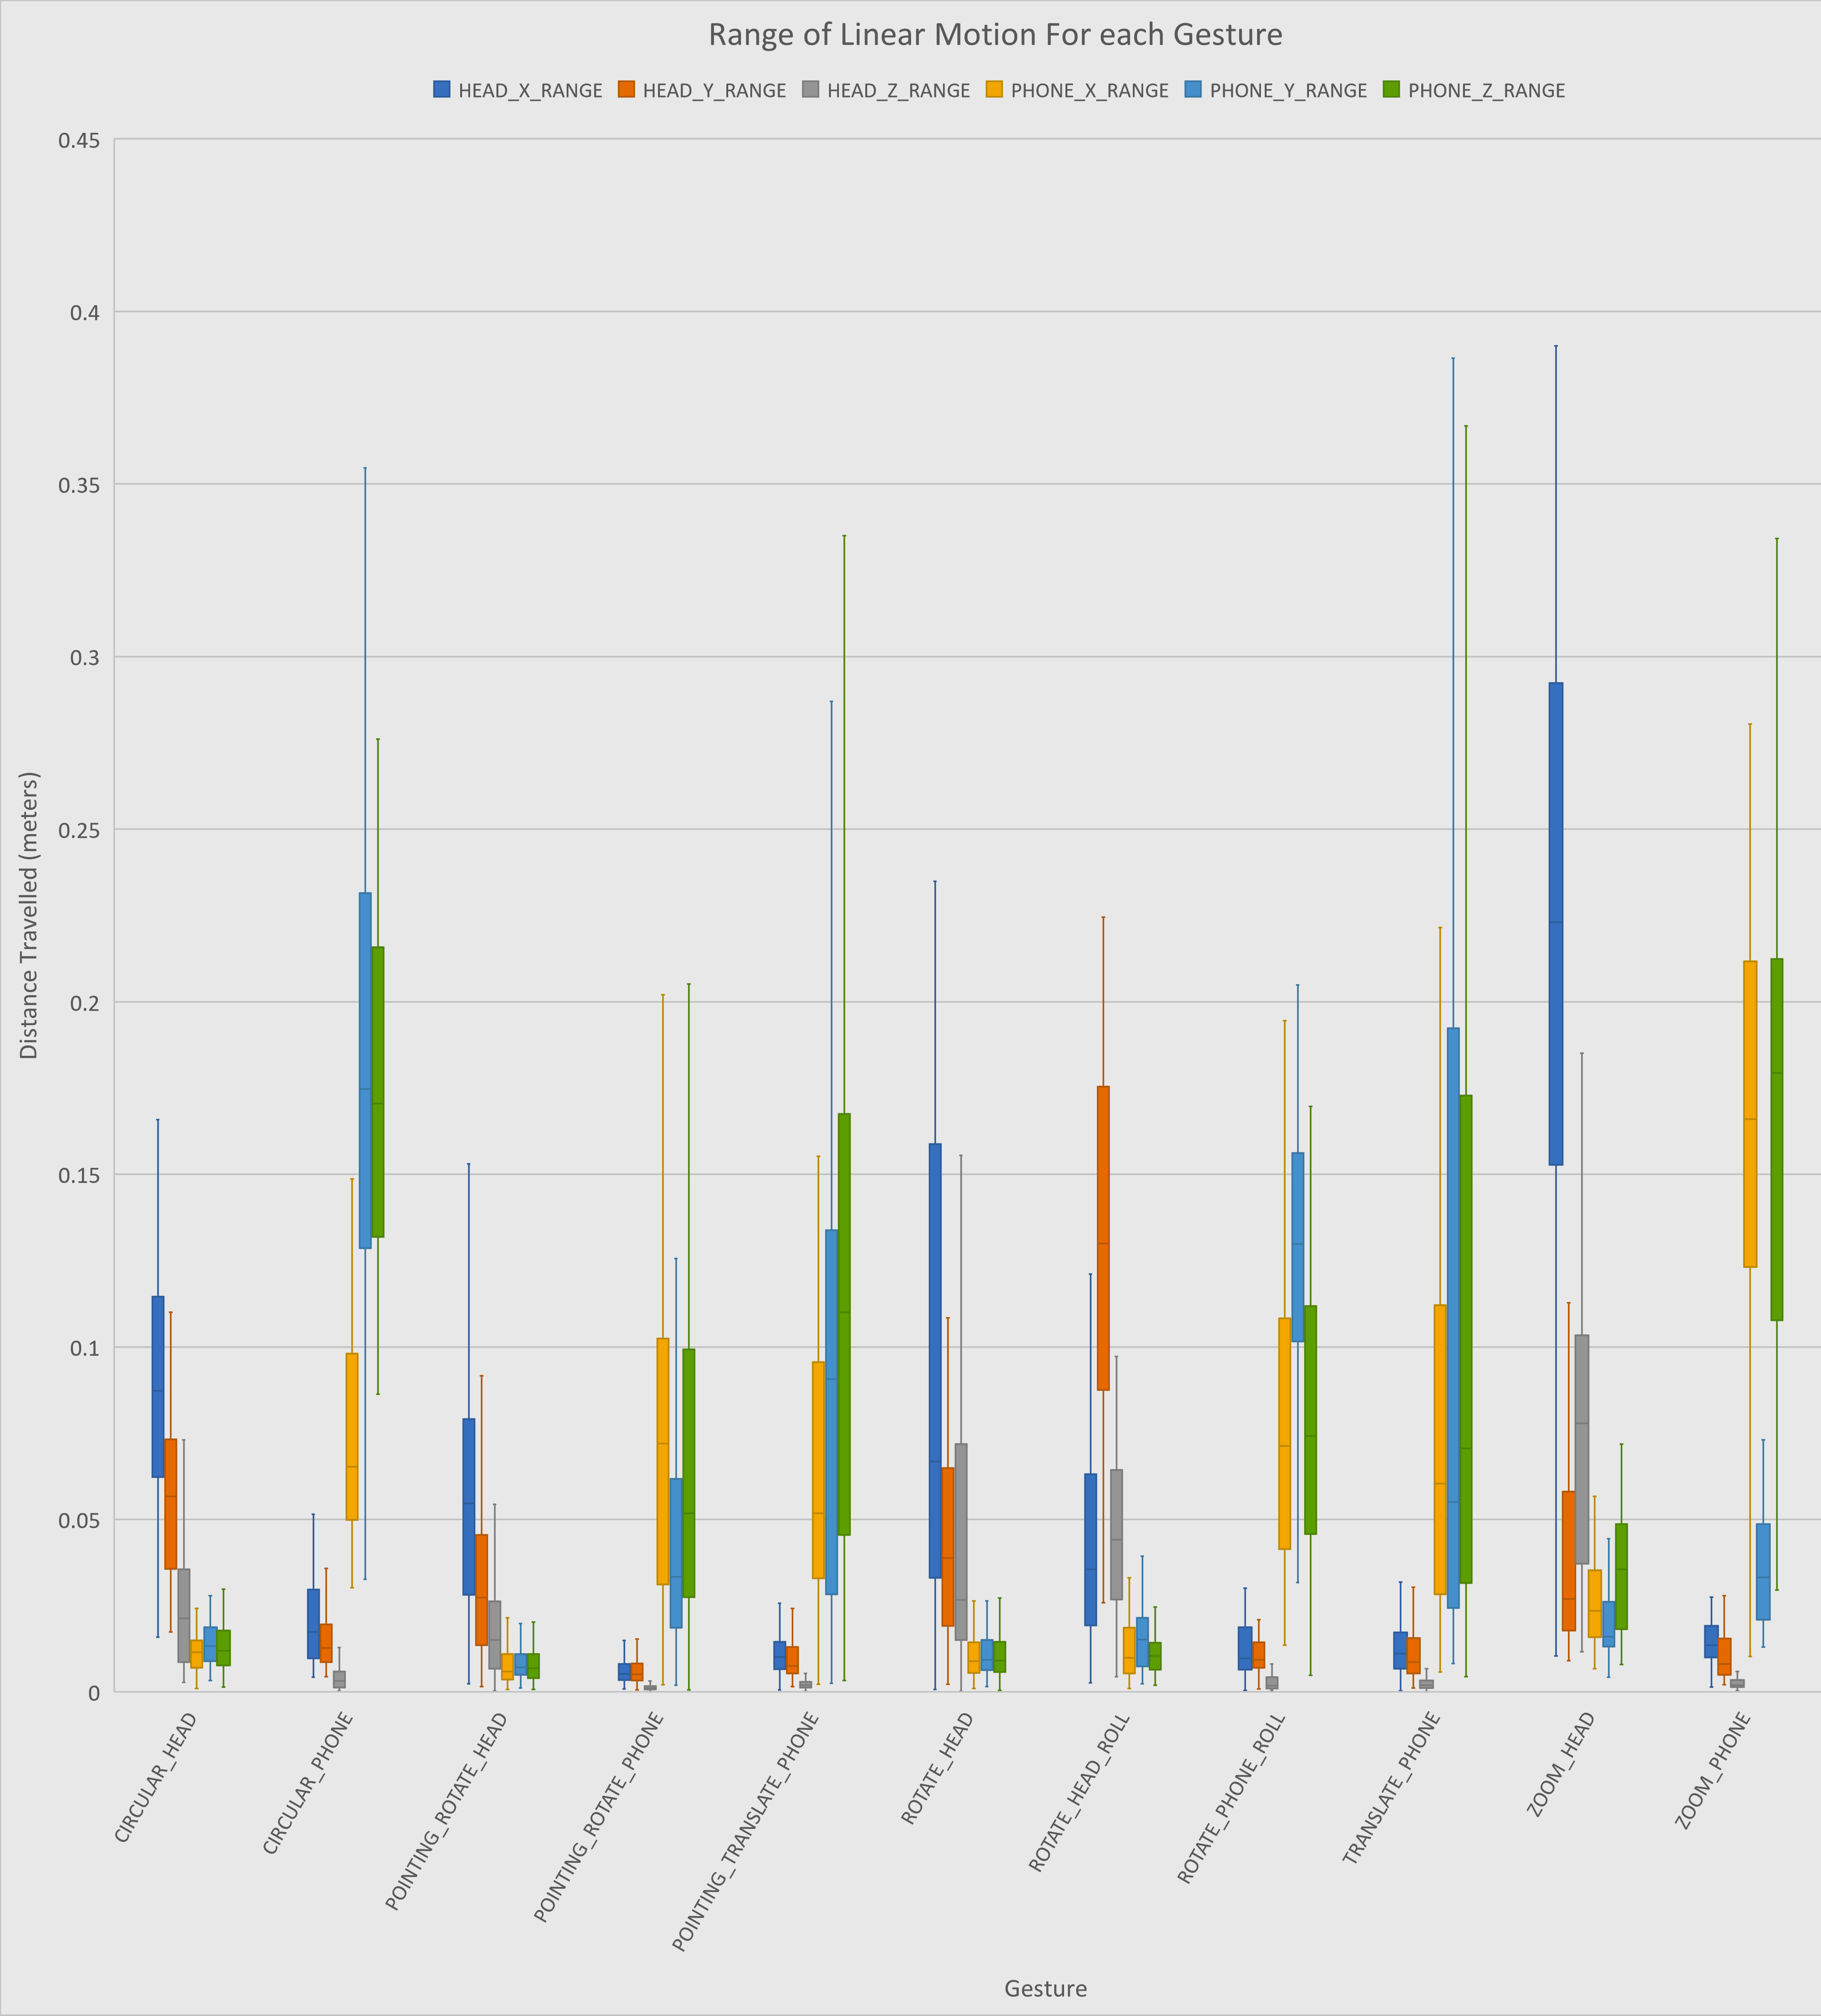
\includegraphics[width=0.9\textwidth]{figures/RangeOfLinearMotion.png}
    \caption{\label{fig:range_of_linear_motion} Range of linear motion for each gesture, in meters}
    \Description{Box and Wisker plot showing the mean, min, max, and the first and third quartiles for the observed range of linear motion for each gesture recorded.}
\end{figure*}
In total we were able to record 1028 gestures. The sample rate for the images was between 30-33 images per second, and the IMU sample rate was an expected 50$Hz$.
A breakdown of the range of linear motion can be seen in \autoref{fig:range_of_linear_motion}.
From this we can see the axis with the greatest movement typically correlate to the object being moved, e.g. the head or the phone, which is to be expected and helps to confirm the MoCap data is accurate.
The gesture with the most movement in any given axis was for moving the head towards and away from the phone, with movement typically being between 15-30cm. However the gestures that involved the most movement across multiple axis were the ones that involved the translation of the phone, which typically saw movement across all three axis.

Unfortunately we are unable to accurately breakdown the range of angular motion as we do not record the amount of rotation performed, only the exact rotation observed. As such we have some issues with rotations being calculated as around 360\textdegree / 2$\pi$. None of the gestures performed by the participants actually required a rotation that large, however due to the cyclical nature of angles, you can rotate a small amount and end up with a larger angle if you try to take the difference between frames. 
This only seems to have impacted the calculation for roll, calculated yaw and pitch appear correct. This is due to the orientation of the participant during recording ensuring that the observed pitch and yaw never exceeding 360\textdegree or falling below 0\textdegree. A breakdown of the angular motion with can be found under \autoref{app:study_data}, however the calculated roll is unfortunately incorrect.
Reviewing the data we do have however does show that the MoCap data is consistent with what we would expect, showing all accurate rotations never exceeding 180\textdegree, rotation being very small during linear motion gestures, and that head gestures typically require greater rotation than those of the phone.

By using a face detector~\cite{yu2022yunet} with OpenCV we were able to generate a breakdown of the percentage of images within which a face could be detected. The percentage of frames with a face detected for each gesture, and variant of a gesture, is available as an appendix under \autoref{app:study_data}, along with a breakdown of average time elapsed performing a gesture. 
From the table we can see that some gestures have much lower frequency of frames wherein the head is detected. Most of these are to be expected, such as the gestures that rotate the phone, which can cause the camera's point of view to no longer include the face. A particular example is the Bottom-Centre variant of the Pointing-Rotate-Phone gesture, which involves the phone being tilted such that the top of the phone is tilted away from the participant's face. Given the front-facing camera is mounted on the top, this will result in the camera moving the furthest from the face.

On average all the gestures took between 2.4 - 3.6 seconds, with the circular and zoom motions, for both head and phone, taking the longest to perform.

    \section{Model Development}
In this section we propose a CNN for encoding the direction of linear and angular movement observed between 2 frames, and a RNN to classify sequences of encoded movement as a gesture.
These models are to be used in tandem to classify semaphoric gestures performed, distinguishing between gesture made with the head and those made with a smartphone.
% script.processor.process_data('G:/Study/7', 1900)
% script.processor.process_data('G:/Study/6', 8900)
% script.processor.process_data('G:/Study/5', 9500)
% script.processor.process_data('G:/Study/4', 900)
% script.processor.process_data('G:/Study/3', 20000)
% script.processor.process_data('G:/Study/2', -320, attempt_0_override=-320)
% script.processor.process_data('G:/Study/1', 1000)
% script.processor.process_data('G:/Study/0', 3000)

% \subsection{The Proposed Models} % TODO: Drop /s if only one model % The Proposed System
% Both models then used to train HMM, evaluate which performs better
% In this section we shall propose two models for quantising the motion of the phone and position of the head, and a HMM to classify sequences of the encoded motion as specific gestures.
% Possibly one-hot encoding
% \nl\textbf{Modularity}\\
% Having a single model do many tasks
We opted to split the development of our model into two distinct models (the CNN and RNN) for 2 reasons.
The first was to reduce the observation space for the RNN, since the acceleration can be any value and the position of the face in the image also any range of values, within the boundaries of the image resolution.
To use them as raw inputs to an RNN would require a significant amount of data to ensure we have samples that cover the entire training space.
By first encoding the data we can reduce the possible training space.
The simplest way to perform this would be to quantise the data. This would involve reducing the resolution of the data, for example mapping all the angles of rotation into a smaller range, as was performed by \citeauthor{elmezain2008hidden} to convert the movement of a hand capture in a sequence of images to the angle of the movement~\cite{elmezain2008hidden}, reducing the possible input to their HMM to just 19 observable states.
We have decided to instead one-hot encode the motion of the head and phone. This reduces the possible states for two frames down to a 12x3 grid, where the columns are the degree of freedom.

The second reason  for the split was to reduce the memory requirements for the system.
An RNN requires a sequence of input in order or to predict an output. If we were to utilise a CNN atop the RNN, we would need to hold enough images in memory for the required input length of the RNN. The longer the input sequence is, the more images we would need. 2 Ways to get around this are to keep a short input sequence, reducing the amount of history that the RNN can learn and predict from; or we can reduce the image size, however reducing them too far can result in fewer features being extractable.
By splitting into two models, with distinct responsibilities, we only need to hold two images at a time in memory to encode the motion, and then hold onto the encodings for the second model's input sequence.

\subsection{Motion Encoding CNN Model}
% Want to reduce the possible observation states we need to learn for our classification HMM.
% \nl\textbfit{Classifier 1}\nl
% 2: Cascading motion encoder
%   No transfer learning
%   use YuNet to preprocess the image. 
%   - If no face found then return no encoding for face
%   - Else feed into NN to encode the motion
%   Acceleration encoded manually, just quantise and see if over given amount, then convert to encoding
\begin{figure*}
    \centering
    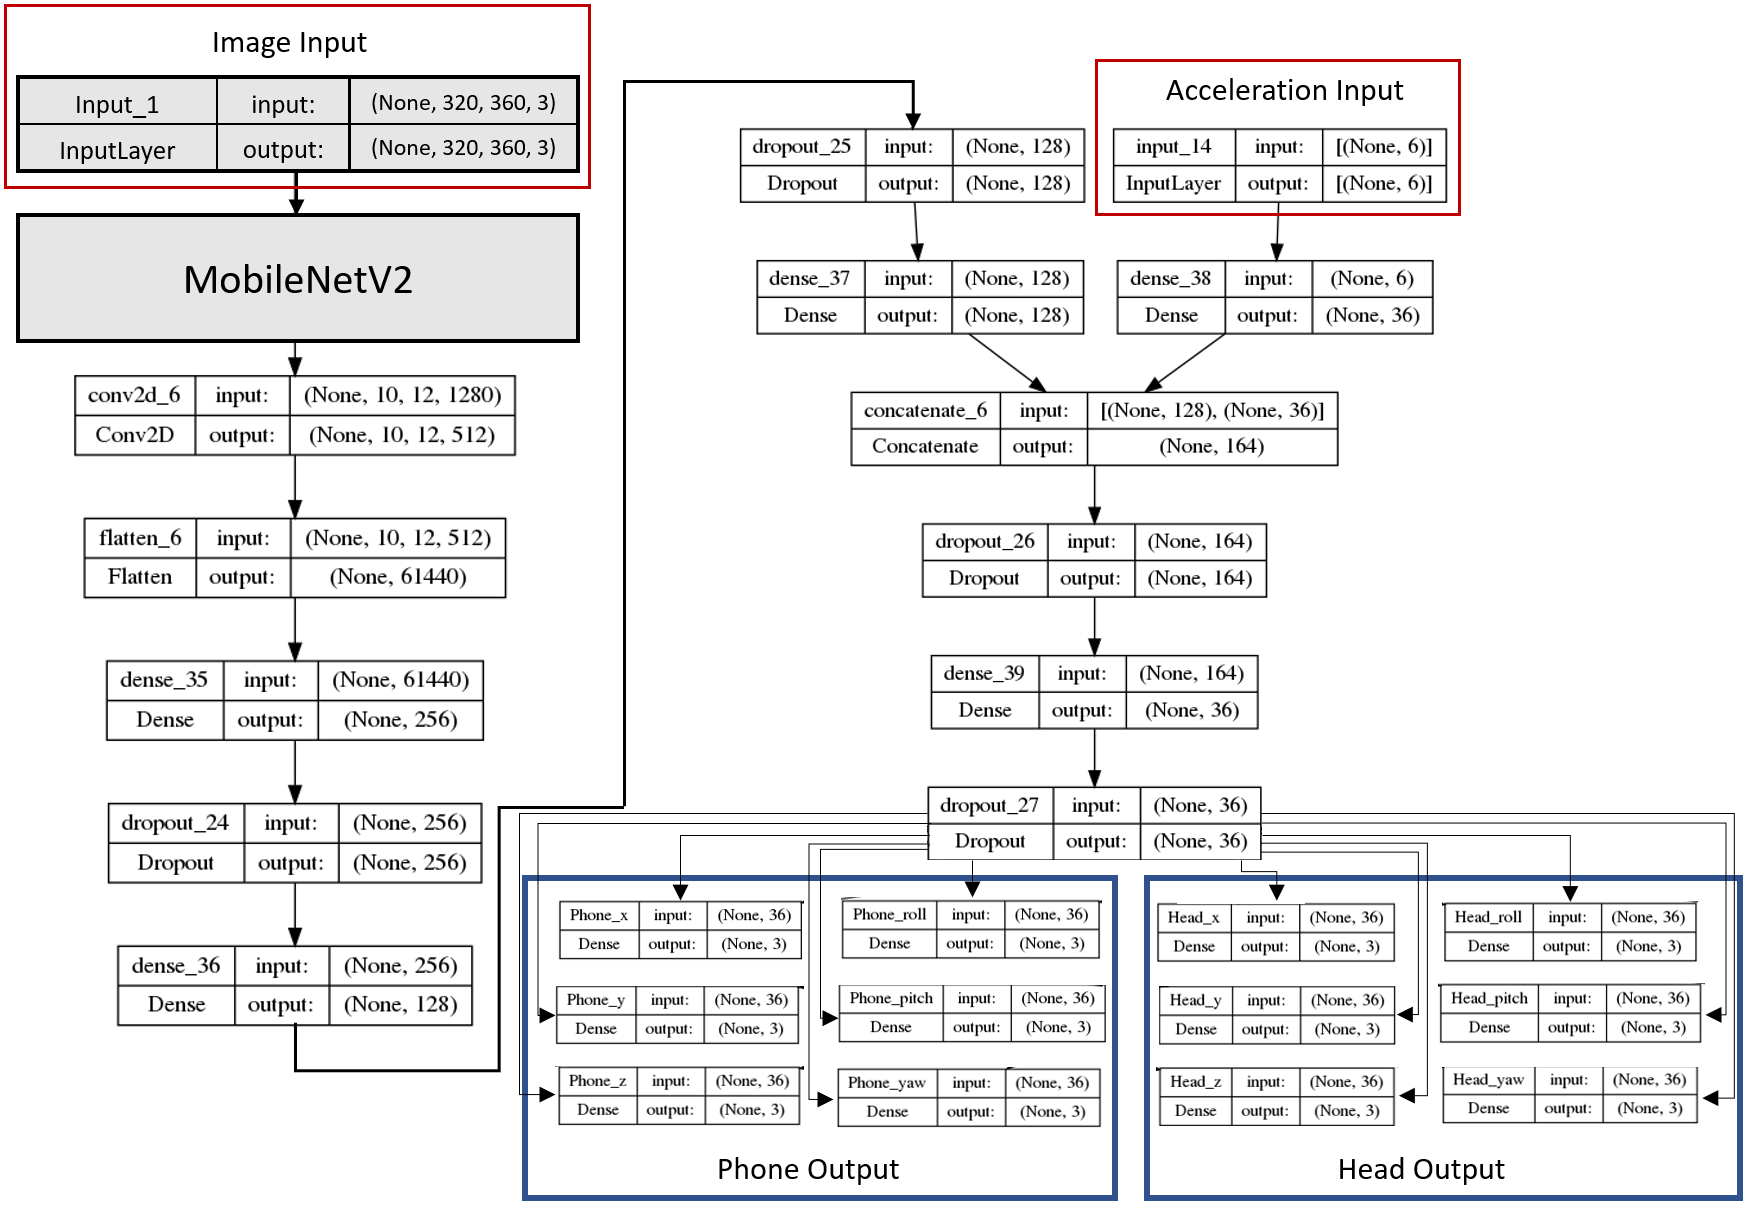
\includegraphics[width=0.95\textwidth]{figures/TL_Model_Clean.png}
    \caption{\label{fig:motion_encoder} Motion Encoder Model}
    \Description{Diagram of the motion encoder model, showing the image inputs feeding into the MobileNetV2 model, the acceleration input being joined with the output of the mobile net and subsequent dense layers, and the 12 expected output.}
\end{figure*}
First we propose a model for extracting the motion performed by the head and the phone.
Since this model requires extracting features from images, in order to learn and predict the motion of the head within the images, we elected to use a CNN.
To save on computation time and effort we employed transfer learning, a technique for extending upon an existing model with pre-initialised weights. For this we chose to use the MobileNetV2 network available within TensorFlow's Keras prebuilt models. We chose MobileNetV2 as, of the models available within Keras\footnote{A list of available models included within Keras for transfer learning can be found here: \url{https://keras.io/api/applications/}}, it strides a balance between size (14MB), accuracy (71.3\%), and CPU step inference time (25.9ms).
MobileNetV2 was trained on the ImageNet dataset\footnote{\url{https://www.image-net.org/}}, a dataset of millions of labelled images. These contain various classes, amongst them are people and faces.
By using just the CNN component of MobileNetV2 and freezing the weights, such that they are not updated during training, we should be able to utilise the features they have already learnt in order to process our image inputs, without needing to train a CNN from scratch.

\begin{figure}
    \centering
    
\includegraphics[width=0.4\textwidth]{figures/concat_input.png}
    \caption{\label{fig:concat_img} Concatenated Image Input For the Motion Encoder}
    \Description{Image composed of two input images that are used as input for the motion encoder.}
\end{figure}
Given we need the model to extract the motion of the head between two images, you may wonder why the input of the model accepts only a single RGB image with the dimensions $320x360x3$, as can be seen in the model graph \autoref{fig:motion_encoder}.
This is due to a limitation of TensorFlow/Keras, wherein using 2 of the same model for transfer learning fails due to layers from each model having the same name, resulting in the model graph being unable to compile. As such we were unable to have two branches utilising the MobileNetV2 to process the images individually. So to get around this issue we first stitch the images side-by-side, such that the older image is on the left, and the later image on the right, as shown in \autoref{fig:concat_img}.
This should not be an issue, as given the nature of CNNs, learned features are not dependent on location within the image, and as such features should still be extracted for both images. This also reduces the size of the model, given it does not need to have two copies of the same CNN.

Following the MobileNetV2 CNN, we add an additional couple of convolution layers, batch normalisation, and max pooling to reduce the parameters in the model, that need to be trained, before flattening the into a 1D tensor that will be concatenated with the acceleration input, starting the first layer of our Fully Connected Network (FCN).
The FCN layers are responsible for performing the classification based on the features extracted in the CNN. 
We opted to provide the acceleration as input into the model in order to allow the model to learn how the head pose changes with respect to acceleration.
We also have the model try to encode the motion of the phone, since we are providing the phone acceleration as input.
The output for this model is a total of 12 layers, each with 3 units which are encoded via a softmax activation function, which normalises the 3 values for each output, such that the most prediction that the model believes is most likely is the value closer to 1.

The model was implemented using TensorFlow's Keras Api.
The full model layers, excluding the MobileNetV2 CNN, can be seen in \autoref{fig:motion_encoder}.

% might encode one-hot instead, in which case take two sequential inputs and calculate the movement

% \nl\textbfit{Classifier 2}\nl
% % 2: NN using transfer learning (using image net model, which one?).
% %   Use tensorflow (work with current cuda and dependencies?) or pytorch?
% %   - 4 inputs, 2 images, 2 sets of acceleration data
% %     Images fed into own image net model, outputs into FCN and then both connected into FCN
% %     Acceleration fed into FCN, then joined with FCN of images
% %   Output one-hot encoded direction of motion for each DoF
% %   might be slow as re-processing previous image
% Our second proposed model we will be using transfer learning to extend an existing CNN trained on image net to predict the direction of motion, in each degree of freedom for both the head and phone, observed between two frames.
% We could try to emulate the YuNet model, and output the head pose and position, a lack of 
% One issue is lack of images not containing face, how to handle if no face detected?


\subsection{Gesture Classification RNN Model}
% Could have used an RNN bolted directly onto the back of the classifiers
\begin{figure}
    \centering
    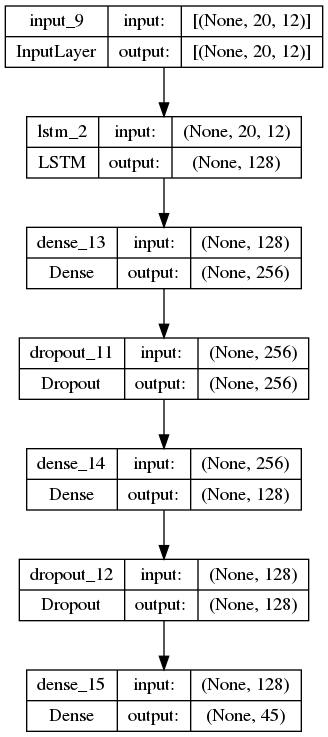
\includegraphics[width=0.25\textwidth]{figures/gesture_model.png}
    \caption{\label{fig:gesture_classifier} Gesture Classifier Model}
    \Description{Diagram of the gesture classifier model, showing the sequence input and one-hot encoded output layers.}
\end{figure}
Once we have our encoded motions, we can now look to classifying the sequence of these observations as gestures.
We elected to use an RNN for this task as, unlike a traditional Neural Network, it can hold onto state between elements of a sequence, allowing it to learn to recognise features within sequences. This is ideal as gesture is a sequence of motions, as long as the motions are correctly encoded and the sequence is long enough to envelop the motion duration, or at least the most significant motions within the gesture.

% \begin{figure}
%     \centering
%     \includegraphics[width=0.45\textwidth]{figures/LSTM.png}
%     \caption{\label{fig:lstm} LSTM Cell Diagram~\cite{phi2018lstm}}
%     \Description{Diagram of the internal structure of an LSTM Cell.}
% \end{figure}
Our proposed gesture classification model, which can bee seen in \autoref{fig:gesture_classifier}, uses a single Long Short Term Memory (LSTM) layer to process the input sequence. An LSTM has two internal states: the hidden state, and the cell state. Both are passed through the chain of cells within the LSTM, with the hidden state being used to represent the prediction of the cell, and the cell state being a means to retain important features from further back in the chain of LSTM cells.
After the LSTM layer the model continues with an FCN with only 3 layers, the layer last being the output of 45 units (1 for each possible gesture from the study, plus no gesture), normalised via a softmax function to one-hot encode the gesture.

As with the first model, this was built using Keras.


% To build and train this we will first collect the output from out first model to generate the training data required. This will give us the data sequences we would expect to see in different gestures.

% How account for different sample rates? How include this as part of observation state?

% If we have no transfer learning
% To achieve our goal we opted to build a model of 3 parts.
% \\\tempnote{Would be 2 parts if can get transfer learning to work, but having issues. Will just leave as preprocessing of the image prior to feeding into model if unable to get it sorted.}\\
% The first stage is to identify if a face is present in an image. For this we utilise a prebuilt CNN which returns a bounding box of the face, along with the points of the eyes, nose, and mouth corners~\cite{yu2022yunet}. %This is executed with OpenCV
% The bounding box and the landmarks, along with the average of the IMU data since the last image, are then passed into a neural network which aims to predict how the head and phone are moving through the 6 Degrees of freedom.
% If no bounding box or landmarks are found for a given image, we provide the previous bounding box and landmarks. Ideally we would not provide anything, however the network expects to 
% \tempnote{is input going to be padded with zeros for first frames / last frames, or require certain number of frames before attempting classification?}\\
% The second model is 2 models which will be trained to predict the direction of movement in each of the 6 DoF for the head and phone (the head model will also take the landmarks and bounding box as input).
% It will output as a 2d one-hot encoded array, each row being the Degree of Freedom, the column being the direction (0 = stationary, -1 = negative, +1 = positive).
% The output of the 2 can then be fed into a HMM trained to predict the gesture performed based on the derived motion. (possibly an RNN if easier)

% What models have been used for cascading (facial landmark and YuNet CNNs)

% Tools, issues

\subsection{Training}
% Breakdown of samples (train, validation, test), and count
Prior to training the first half of proposed model, we wanted to increase the amount of effective data we have for training we performed some fps scaling of the data. 
This involved iterating through our collected data and only extracting frames if they \textit{would} have been available at a lower sample rate. 
For example, if we had 60 images sampled at 30fps and wanted to treat the data like it was at 10fps, we would wind-up with a sequence of 20 images sampled from the original 60.

For the images and the MoCap data we simply took the last available datum for the current new timestamp, but for the accelerations we calculated the average based on the time elapsed, as using just the last value would not be representative of the acceleration of the phone during the period.
Additionally if a second image were to occur before the expected, for the given frame-rate, we would create a new file starting at this image, with the intention that we could generate an additional set of data from the same recording, but offset slightly, ensuring the lower sample rates are still processing all of the images captured during the study.
In deployment of the model this would require that the accelerations are averaged in between images being captured, but this should provide greater resolution on how the phone is moving.

As a result of this resampling of the collected data, we were able to generate the following:
\begin{description}
    \item[Raw] - 1029 gesture recordings without resampling, recorded at about 32fps.
    \item[5 fps] - 7997 gesture recordings sampled.
    \item[10 fps] - 4971 gesture recordings sampled.
    \item[15 fps] - 4451 gesture recordings sampled.
    \item[20 fps] - 4184 gesture recordings sampled.
\end{description}
During our generation of the resampled data, we also generated the expected motion encoding for each pair of frames for a given sample rate by quantising the mocap data, reducing the rotation range from 360\textdegree to -9 to 9 and converting the positional data from metres to centimetres and rounding to the nearest int. We then generated encodings such that \verb|[1,0,0]| indicates a negative delta, \verb|[0,1,0]| no delta, and \verb|[0,0,1]| indicating a positive delta.

Both models were trained on the same machine, which was equipped with an Nvidia Geforce RTX 3070 GPU with 8GB of dedicated video memory, 32GB of RAM, and an Intel i5-10600K CPU.
The Motion Encoder model was trained using the GPU, unfortunately the Gesture Classification model was run with only the CPU due to an issue that developed between training the models which resulted in a failure to load required CUDA libraries. 

The Motion Encoder was trained on only a subset of the full training data generated as the initial epoch runtime estimate was over 48hrs. As such we chose to instead use the 10 fps resampled data, as it still contained over 170k motion encodings to learn, within the 4971 resamples.

The Gesture Classifier was trained on the same subset of data, however the only data from the files extracted were the motion encodings as input, and the file names used as the gesture class. The gesture class was also one-hot encoded.
We chose to train the second model using the encoded motion data generated during the resampling, rather than using data generated from the output of the first model, to ensure that it was trained on ideal and expected data. This way if the first model was unable to accurately predict motion, we would still be able to verify whether using an RNN to learning from a sequence of encoded motion could still be effective at classifying gestures.
An further difference to the input for our second model is that it takes a sequence of input. To generate these we read-in all the gesture recordings, shuffle the order of the recordings. Once we have our shuffled recordings we read from the first frame for the required length of the input sequence and extract this as a single input sequence before starting from the second frame and repeat, resulting in over-lapping sequences. If the length of a recording, from the current frame, is shorter than the required sequence length, we capture until the end of the that recording and begin reading frames from the next recording. 

We elected to merge together different recordings into sequences as we did not want to expect the input of the model to be a clean sample of motion from a single gesture, as this would require additional pre-processing to segment input. instead
If a sequence contained input from more than one recording, we set the class to be whichever gesture had the most frames within the recording. We did originally try to derive the average encoding, however this would not work with Categorical Cross Entropy loss calculations, and would prevent the model from learning.

During the generation of the input sequences we also extracted sequences motions encodings which had all degrees of motion encoded as being stationary. This was because we unfortunately failed to include a stationary gesture in our study, e.g. a recording of the participants not performing any gesture. A model learns to only predict gestures is thusly going to be incorrect whenever a gesture is not being performed. This also removed the stationary sequences prior to or after participants performed the gesture during recordings.

% Only 10 \& 15 fps files Number of files to process: 9422 - Testing paths: 1885, Training: 6029, Validation: 1508
% \tempnote{Additionally generated the required classification output for the motion encoders.}
% Only 10 fps files Number of files to process: 4971 Testing paths: 995, Training: 3180, Validation: 796

% 1028 recordings of gestures.
% K-Fold validation

% Hyper-params (quantisation, image size (if transfer learning?), fps scales)
% Image input sizes


    % How will be evaluated?
% Given the app, how will we evaluate it (setup tasks and verify success rate?)

\section{Model Evaluation} % < 1 Page
% Raw results, table of stats, some analysis (e.g. success rate)
In this section we display the results of our model evaluation.
These results include the training and validation loss, along with the confusion matrices for the models when run against the testing set that they were not trained on.

\subsection{Motion Encoder}
\begin{figure}
    \centering
    \includegraphics[width=0.4\textwidth]{figures/motion_acc_tall.png}
    \caption{\label{fig:motion_encoder_acc} Motion Encoder Validation Loss and Accuracy}
    \Description{Chart showing the accuracy of the motion encoder model during training.}
\end{figure}
During training and validation of the motion encoder, we observed only slight improvement in the encoders accuracy for all the linear axes, and rotational axes showing greater than 70\% accuracy from the first epoch, with very little change as training progresses, see \autoref{fig:motion_encoder_acc}.

\begin{figure}
    \centering
    \includegraphics[width=0.5\textwidth]{figures/motion_encoder_cm.png}
    \caption{\label{fig:motion_encoder_cm} Motion Encoder Confusion Matrix From Testing Set Evaluation}
    \Description{Confusion matrix for the motion encoder using testing set as input}
\end{figure}
A confusion matrix created by comparing model predictions against our testing set, shown in \autoref{fig:motion_encoder_cm}, shows that for the majority of outputs the encoding predicted is for no movement. Of the 12 outputs only Phone X, Y, \& Z, and Head X made predictions for non-stationary movement, and of those only Phone Y showed predictions of negative movement.

\subsection{Gesture Classifier}
\begin{figure}
    \centering
    \includegraphics[width=0.4\textwidth]{figures/gesture_acc_tall.png}
    \caption{\label{fig:gesture_classifier_acc} Gesture Classifier Training and Validation Loss and Accuracy}
    \Description{Chart showing the accuracy of the motion encoder model during training.}
\end{figure}
During training and validation of the gesture classifier, we observe accuracy an loss plateauing from the tenth epoch, as seen in \autoref{fig:gesture_classifier_acc}.

\begin{figure*}
    \centering
    \includegraphics[width=0.9\textwidth]{figures/gesture_confusion.png}
    \caption{\label{fig:gesture_classifier_cm} Gesture Classifier Confusion Matrix From Testing Set Evaluation}
    \Description{Confusion matrix for the gesturew classifer using testing set as input}
\end{figure*}
Reviewing the confusion matrix for the gesture classifier (\autoref{fig:gesture_classifier_cm}) shows a high number of No Gesture samples and predictions, with a clearly defined set of true positives down the diagonal, with only minor noise throughout the rest of the matrix. The low values for the noise could however be slightly distorted by the high number of No Gestures sampled.
% NO\_GESTURE - Predicted: 16913, Actual: 14611, TP: 5516, TN: 62684, FP: 9095, FN: 11397, ACC: 0.7689532314075678, PREC: 0.3775237834508247, REC: 0.32613965588600485, SPEC: 0.8732916312570529, F1: 0.3499555893922091
% POINTING\_TRANSLATE\_PHONE\_TOP\_CENTRE - Predicted: 1632, Actual: 2076, TP: 1054, TN: 90500, FP: 1022, FN: 578, ACC: 0.9828241406702879, PREC: 0.5077071290944123, REC: 0.6458333333333334, SPEC: 0.9888332859858832, F1: 0.5685005393743258
% POINTING\_TRANSLATE\_PHONE\_TOP\_RIGHT - Predicted: 2010, Actual: 2161, TP: 1369, TN: 90037, FP: 792, FN: 641, ACC: 0.9845646764829435, PREC: 0.6335030078667284, REC: 0.6810945273631841, SPEC: 0.9912803179601228, F1: 0.6564373052025894
% POINTING\_TRANSLATE\_PHONE\_MID\_RIGHT - Predicted: 1281, Actual: 1346, TP: 853, TN: 91581, FP: 493, FN: 428, ACC: 0.9901344330780355, PREC: 0.6337295690936107, REC: 0.6658860265417642, SPEC: 0.9946456111388665, F1: 0.6494099733536353
% POINTING\_TRANSLATE\_PHONE\_BOTTOM\_RIGHT - Predicted: 1397, Actual: 1402, TP: 890, TN: 91409, FP: 512, FN: 507, ACC: 0.9890803489144645, PREC: 0.6348074179743224, REC: 0.6370794559770938, SPEC: 0.9944299996736328, F1: 0.6359414076455877
% POINTING\_TRANSLATE\_PHONE\_BOTTOM\_CENTRE - Predicted: 1729, Actual: 2457, TP: 1064, TN: 90022, FP: 1393, FN: 665, ACC: 0.9779051790775574, PREC: 0.43304843304843305, REC: 0.6153846153846154, SPEC: 0.9847618005797736, F1: 0.5083612040133779
% POINTING\_TRANSLATE\_PHONE\_BOTTOM\_LEFT - Predicted: 1739, Actual: 2048, TP: 1143, TN: 90421, FP: 905, FN: 596, ACC: 0.9838714876699082, PREC: 0.55810546875, REC: 0.6572742955721679, SPEC: 0.9900904452182292, F1: 0.6036440454185371
% POINTING\_TRANSLATE\_PHONE\_MID\_LEFT - Predicted: 1763, Actual: 1597, TP: 947, TN: 90848, FP: 650, FN: 816, ACC: 0.9842806746657231, PREC: 0.5929868503443957, REC: 0.5371525808281339, SPEC: 0.9928960195851275, F1: 0.5636904761904762
% POINTING\_TRANSLATE\_PHONE\_TOP\_LEFT - Predicted: 2194, Actual: 1641, TP: 1240, TN: 90373, FP: 401, FN: 954, ACC: 0.9854250925049479, PREC: 0.7556368068251066, REC: 0.5651777575205105, SPEC: 0.9955824354991517, F1: 0.6466753585397653
% POINTING\_ROTATE\_PHONE\_TOP\_CENTRE - Predicted: 2043, Actual: 1339, TP: 986, TN: 90826, FP: 353, FN: 1057, ACC: 0.9848748149578426, PREC: 0.736370425690814, REC: 0.48262359275575134, SPEC: 0.99612849449983, F1: 0.5830869308101715
% POINTING\_ROTATE\_PHONE\_TOP\_RIGHT - Predicted: 1609, Actual: 1940, TP: 1303, TN: 90659, FP: 637, FN: 306, ACC: 0.9898498466175125, PREC: 0.6716494845360824, REC: 0.8098197638284649, SPEC: 0.9930226954083421, F1: 0.7342913496759651
% POINTING\_ROTATE\_PHONE\_MID\_RIGHT - Predicted: 1735, Actual: 1608, TP: 1173, TN: 90865, FP: 435, FN: 562, ACC: 0.9892836029451282, PREC: 0.7294776119402985, REC: 0.6760806916426513, SPEC: 0.9952354874041621, F1: 0.7017648818426563
% POINTING\_ROTATE\_PHONE\_BOTTOM\_RIGHT - Predicted: 990, Actual: 1527, TP: 716, TN: 91691, FP: 811, FN: 274, ACC: 0.9883947289607667, PREC: 0.46889325474787164, REC: 0.7232323232323232, SPEC: 0.9912326219973622, F1: 0.5689312673818037
% POINTING\_ROTATE\_PHONE\_BOTTOM\_CENTRE - Predicted: 1896, Actual: 1917, TP: 1374, TN: 90395, FP: 543, FN: 522, ACC: 0.988527910032962, PREC: 0.7167449139280125, REC: 0.7246835443037974, SPEC: 0.9940288988101784, F1: 0.7206923682140047
% POINTING\_ROTATE\_PHONE\_BOTTOM\_LEFT - Predicted: 1171, Actual: 1144, TP: 781, TN: 91893, FP: 363, FN: 390, ACC: 0.99194023141062, PREC: 0.6826923076923077, REC: 0.6669513236549958, SPEC: 0.996065296566077, F1: 0.6747300215982722
% POINTING\_ROTATE\_PHONE\_MID\_LEFT - Predicted: 2033, Actual: 1930, TP: 1407, TN: 90245, FP: 523, FN: 626, ACC: 0.9876186679022856, PREC: 0.7290155440414507, REC: 0.692080668962125, SPEC: 0.994238057465186, F1: 0.7100681302043907
% POINTING\_ROTATE\_PHONE\_TOP\_LEFT - Predicted: 1577, Actual: 1834, TP: 1346, TN: 90797, FP: 488, FN: 231, ACC: 0.9922573280782236, PREC: 0.7339149400218102, REC: 0.8535193405199747, SPEC: 0.9946541052746891, F1: 0.7892113749633538
% POINTING\_ROTATE\_HEAD\_TOP\_CENTRE - Predicted: 1420, Actual: 1431, TP: 899, TN: 91357, FP: 532, FN: 521, ACC: 0.9887149149599717, PREC: 0.6282320055904962, REC: 0.6330985915492958, SPEC: 0.9942104060333663, F1: 0.630655910206945
% POINTING\_ROTATE\_HEAD\_TOP\_RIGHT - Predicted: 1427, Actual: 1763, TP: 947, TN: 91018, FP: 816, FN: 480, ACC: 0.9861035159391386, PREC: 0.5371525808281339, REC: 0.6636299929922915, SPEC: 0.9911144020733061, F1: 0.5937304075235109
% POINTING\_ROTATE\_HEAD\_MID\_RIGHT - Predicted: 1272, Actual: 1324, TP: 912, TN: 91612, FP: 412, FN: 360, ACC: 0.9917252615331847, PREC: 0.6888217522658611, REC: 0.7169811320754716, SPEC: 0.9955229070677215, F1: 0.7026194144838213
% POINTING\_ROTATE\_HEAD\_BOTTOM\_RIGHT - Predicted: 1265, Actual: 1534, TP: 794, TN: 91409, FP: 740, FN: 471, ACC: 0.9870362044233199, PREC: 0.5176010430247718, REC: 0.6276679841897234, SPEC: 0.9919695276128878, F1: 0.5673454805287603
% POINTING\_ROTATE\_HEAD\_BOTTOM\_CENTRE - Predicted: 1032, Actual: 1219, TP: 672, TN: 91957, FP: 547, FN: 360, ACC: 0.9903031987683887, PREC: 0.5512715340442986, REC: 0.6511627906976745, SPEC: 0.9940867421949321, F1: 0.5970679697912039
% POINTING\_ROTATE\_HEAD\_BOTTOM\_LEFT - Predicted: 1173, Actual: 1281, TP: 849, TN: 91754, FP: 432, FN: 324, ACC: 0.9919022268876059, PREC: 0.6627634660421545, REC: 0.7237851662404092, SPEC: 0.9953138220554097, F1: 0.6919315403422983
% POINTING\_ROTATE\_HEAD\_MID\_LEFT - Predicted: 1790, Actual: 1906, TP: 1310, TN: 90512, FP: 596, FN: 480, ACC: 0.9884174040345325, PREC: 0.6873032528856243, REC: 0.7318435754189944, SPEC: 0.993458313210695, F1: 0.7088744588744589
% POINTING\_ROTATE\_HEAD\_TOP\_LEFT - Predicted: 1510, Actual: 1558, TP: 1127, TN: 91140, FP: 431, FN: 383, ACC: 0.9912549285031317, PREC: 0.7233632862644416, REC: 0.7463576158940397, SPEC: 0.9952932697032904, F1: 0.7346805736636245
% TRANSLATE\_PHONE\_TOP\_CENTRE - Predicted: 1494, Actual: 1340, TP: 830, TN: 91374, FP: 510, FN: 664, ACC: 0.9874274454368267, PREC: 0.6194029850746269, REC: 0.5555555555555556, SPEC: 0.9944495233120021, F1: 0.5857445306986592
% TRANSLATE\_PHONE\_MID\_RIGHT - Predicted: 2023, Actual: 1636, TP: 1155, TN: 90549, FP: 481, FN: 868, ACC: 0.9855028854523766, PREC: 0.7059902200488998, REC: 0.5709342560553633, SPEC: 0.9947160276831813, F1: 0.6313200327958459
% TRANSLATE\_PHONE\_BOTTOM\_CENTRE - Predicted: 1989, Actual: 1905, TP: 1178, TN: 90314, FP: 727, FN: 811, ACC: 0.9834676985918521, PREC: 0.6183727034120735, REC: 0.5922574157868276, SPEC: 0.9920145868345032, F1: 0.6050333846944016
% TRANSLATE\_PHONE\_MID\_LEFT - Predicted: 1478, Actual: 1682, TP: 1068, TN: 91048, FP: 614, FN: 410, ACC: 0.9890057977238566, PREC: 0.6349583828775267, REC: 0.7225981055480379, SPEC: 0.9933014771661103, F1: 0.6759493670886076
% CIRCULAR\_PHONE\_CLOCKWISE - Predicted: 2845, Actual: 3177, TP: 1961, TN: 88186, FP: 1216, FN: 884, ACC: 0.9772350320335621, PREC: 0.6172489770223482, REC: 0.6892794376098418, SPEC: 0.986398514574618, F1: 0.6512786449684489
% CIRCULAR\_PHONE\_ANTI\_CLOCKWISE - Predicted: 2231, Actual: 1793, TP: 1369, TN: 90184, FP: 424, FN: 862, ACC: 0.9861480627753423, PREC: 0.7635248187395427, REC: 0.6136261766024205, SPEC: 0.9953205015009712, F1: 0.6804174950298211
% CIRCULAR\_HEAD\_CLOCKWISE - Predicted: 2003, Actual: 1984, TP: 1370, TN: 90221, FP: 614, FN: 633, ACC: 0.9865680001723433, PREC: 0.6905241935483871, REC: 0.6839740389415876, SPEC: 0.9932404910001651, F1: 0.6872335089039378
% CIRCULAR\_HEAD\_ANTI\_CLOCKWISE - Predicted: 1976, Actual: 2301, TP: 1498, TN: 89931, FP: 803, FN: 478, ACC: 0.9861827203106461, PREC: 0.6510212950890917, REC: 0.7580971659919028, SPEC: 0.9911499548129697, F1: 0.7004909983633387
% ZOOM\_PHONE\_ZOOM\_IN - Predicted: 2652, Actual: 2326, TP: 1595, TN: 89230, FP: 731, FN: 1057, ACC: 0.9806938550743416, PREC: 0.6857265692175408, REC: 0.6014328808446455, SPEC: 0.9918742566223141, F1: 0.6408196062675774
% ZOOM\_PHONE\_ZOOM\_OUT - Predicted: 2002, Actual: 1705, TP: 1215, TN: 90501, FP: 490, FN: 787, ACC: 0.9862677835966148, PREC: 0.7126099706744868, REC: 0.6068931068931069, SPEC: 0.9946148520183314, F1: 0.6555165902346911
% ZOOM\_HEAD\_ZOOM\_IN - Predicted: 2213, Actual: 1970, TP: 1600, TN: 90025, FP: 370, FN: 613, ACC: 0.9893853662750518, PREC: 0.8121827411167513, REC: 0.7230004518752824, SPEC: 0.9959068532551579, F1: 0.7650011953143677
% ZOOM\_HEAD\_ZOOM\_OUT - Predicted: 1676, Actual: 1886, TP: 1233, TN: 90646, FP: 653, FN: 443, ACC: 0.9882118849152998, PREC: 0.6537645811240721, REC: 0.7356801909307876, SPEC: 0.9928476763162795, F1: 0.6923076923076924
% ROTATE\_HEAD\_TOP\_CENTRE - Predicted: 2135, Actual: 2367, TP: 1372, TN: 89706, FP: 995, FN: 763, ACC: 0.9810633805851179, PREC: 0.5796366708914238, REC: 0.6426229508196721, SPEC: 0.9890298894168752, F1: 0.6095068858285206
% ROTATE\_HEAD\_MID\_RIGHT - Predicted: 2158, Actual: 2024, TP: 1409, TN: 90026, FP: 615, FN: 749, ACC: 0.9853015657496309, PREC: 0.6961462450592886, REC: 0.6529193697868396, SPEC: 0.993214991008484, F1: 0.6738402678144428
% ROTATE\_HEAD\_BOTTOM\_CENTRE - Predicted: 1729, Actual: 2074, TP: 1288, TN: 90405, FP: 786, FN: 441, ACC: 0.9867950925527336, PREC: 0.6210221793635486, REC: 0.7449392712550608, SPEC: 0.9913807283613515, F1: 0.6773599789639757
% ROTATE\_HEAD\_MID\_LEFT - Predicted: 2066, Actual: 2592, TP: 1693, TN: 89550, FP: 899, FN: 373, ACC: 0.9862508782359617, PREC: 0.6531635802469136, REC: 0.81945788964182, SPEC: 0.9900606971884709, F1: 0.7269214255045084
% ROTATE\_PHONE\_ROLL\_CLOCKWISE - Predicted: 1685, Actual: 1982, TP: 1466, TN: 90541, FP: 516, FN: 219, ACC: 0.9920747881218865, PREC: 0.739656912209889, REC: 0.8700296735905044, SPEC: 0.994333219851302, F1: 0.7995636760294519
% ROTATE\_PHONE\_ROLL\_ANTI\_CLOCKWISE - Predicted: 1862, Actual: 1753, TP: 1554, TN: 90593, FP: 199, FN: 308, ACC: 0.9945280290111598, PREC: 0.8864803194523674, REC: 0.8345864661654135, SPEC: 0.9978081769318883, F1: 0.8597510373443984
% ROTATE\_HEAD\_ROLL\_CLOCKWISE - Predicted: 1934, Actual: 1816, TP: 1433, TN: 90458, FP: 383, FN: 501, ACC: 0.99047157100512, PREC: 0.7890969162995595, REC: 0.7409513960703206, SPEC: 0.9957838420977312, F1: 0.7642666666666666
% ROTATE\_HEAD\_ROLL\_ANTI\_CLOCKWISE - Predicted: 1456, Actual: 1301, TP: 1121, TN: 91451, FP: 180, FN: 335, ACC: 0.9944675411174493, PREC: 0.8616448885472713, REC: 0.7699175824175825, SPEC: 0.9980355993059118, F1: 0.8132027566195139


    \section{Discussion} % < 1 Page
% How did models perform, what motions / gestures were difficult
% Which model performed best

% What do the results mean?
% Why might the cause of some of the issues be?
% Was this a success or failure?

% Performance, how long to run models?
% How did models perform deployed compared to confusion matrices (did those with bad CM perform better than others?)
% NN Vs Other methods


% What do the results mean?
% Why might the cause of some of the issues be?
% Was this a success or failure?


\subsection{Limitations and Further Work} % < 0.5 Pages
% What should be done to improve
% Collect more data (to improve accuracy)
% no images that do not contain a face (at least no labelled images as such. could use existing Android MLKit tools to cascade and ignore sequences over 20 frames without a head)
% only trained at 10fps, if gesture takes longer than 2 seconds, could fail to be accurately detected

% What were the limitations with the data collection / system developed?

% Retrain with different hyper-params ()


% Further work
Depending on the model limited by only recognising gestures, not pointing / cursor manipulation
% improve model for motion encoding, possibly utilise kalman filters, or an alternative preprocessing of the accelerations to help improve motion encoding for linear acceleration.

% Integrate into smartphone app and measure performance

    \section{Conclusion} % < 0.5 Pages
% Summarise what was discussed within the paper, and what was contributed.

    
    \bibliographystyle{styling/bibliography/ACM-Reference-Format} % bath-harvard?
    \bibliography{sections/references}
    
    \appendix
% Tell TexCount to ignore words in word count
%TC:ignore
\clearpage
\restoregeometry
\newpage
\section{Table of Gestures and Variations}\label{app:gestures}
\textbf{Head Gestures}
\begin{description}
    \item[Pointing-Rotate]\nl
    Turn your head such that the desired content is in the centre of your vision. E.g. if the target is in the bottom right corner of the screen, turn your head down and to the right\\
    \textbfit{Directions:} Up, Up-Right, Right, Down-Right, Down, Down-Left, Left, Up-Left
    \item[Circular]\nl
    Turn your head such that the path of motion of your nose draws a circle.\\
    \textbfit{Directions:} Clockwise, Anti-Clockwise
    \item[Zoom]\nl
    Move your head directly towards or away from the phone screen.\\
    \textbfit{Directions:} Zoom-In, Zoom-Out
    \item[Rotate]\nl
    Turn your head such that you are looking beyond the edge of the screen.\\
    \textbfit{Directions:} Up, Right, Down, Left
    \item[Roll]\nl
    Lean your head to the left or right, bringing it towards your shoulder.\\
    \textbfit{Directions:} Clockwise (Right), Anti-Clockwise (Left)
\end{description}\nl
\textbf{Phone Gestures}
\begin{description}
    \item[POINTING-TRANSLATE]\nl
    Move the phone such that the desired content is in the centre of your vision. E.g. if the target is in the bottom right corner of the screen, move the phone up and to the left.\\
    \textbfit{Directions:} Up, Up-Right, Right, Down-Right, Down, Down-Left, Left, Up-Left
    \item[POINTING-ROTATE]\nl
    Turn the phone such that the desired content is in the centre of your vision. E.g. if the target is in the bottom right corner of the screen, twist the phone such that the bottom right corner is brought towards your face.\\
    \textbfit{Directions:} Up, Up-Right, Right, Down-Right, Down, Down-Left, Left, Up-Left
    \item[Translate]\nl
    Move the phone such that the phone is off to the side of your head.\\
    \textbfit{Directions:} Up, Right, Down, Left
    \item[Circular]\nl
    Move the phone such that its path of motion draws a circle.\\
    \textbfit{Directions:} Clockwise, Anti-Clockwise
    \item[Zoom]\nl
    Move the phone directly towards or away from your head.\\
    \textbfit{Directions:} Zoom-In, Zoom-Out
    \item[Roll]\nl
    Twist the phone such that the phone centre is still the same location, but the corners of the phone are moving clockwise or anti-clockwise.\\
    \textbfit{Directions:} Clockwise, Anti-Clockwise
\end{description}
% \begin{table}[H]
%     \centering
%     \caption{Breakdown of Participants}
%     \label{tab:gesture_breakdown}
%     \begin{tabular}{ c | c | c }
%         Gesture & Description & Directions \\
%         \hline
%         POINTING-TRANSLATE-PHONE & 23 & \\
%         1 & 25 & \\
%         2 & 21 & \\
%         3 & 24 & \\
%         4 & 26 & \\
%         5 & 24 & \\
%         6 & 27 & \\
%         7 & 23 & \\
%         \hline
%     \end{tabular}
% \end{table}

% Data Collection App PUML
% \section{Data Collection App Class Diagram}
% \tempnote{puml sequence diagram showing study steps}

% Full Study Protocol
% \section{Study Protocol Diagram}\label{app:protocol}
% \tempnote{puml sequence diagram showing study steps}
\newpage
\section{Study Data Analysis}\label{app:study_data}
\begin{table}
    \centering
    \caption{Frames with head visible, and total time elapsed per gesture and direction}
    \label{tab:gesture_analysis}
    \begin{tabular}{ c | c | c }
        Gesture And Direction & Percentage of Frames Where Head Is Detected & Time Elapsed (seconds) \\
        \hline
        \textbf{CIRCULAR-HEAD} & \textbfit{97.4\%} & \textbfit{3.208} \\
        ANTI-CLOCKWISE & 97.1\% & 3.156 \\
        CLOCKWISE & 97.7\% & 3.261 \\
        \hline
        \textbf{CIRCULAR-PHONE} & \textbfit{96.1\%} & \textbfit{3.618} \\
        ANTI-CLOCKWISE & 95.9\% & 3.451 \\
        CLOCKWISE & 96.4\% & 3.785 \\
        \hline
        \textbf{POINTING-ROTATE-HEAD} & \textbfit{97.2\%} & \textbfit{2.466} \\
        BOTTOM-CENTRE & 95.3\% & 2.489 \\
        BOTTOM-LEFT & 99.9\% & 2.522 \\
        BOTTOM-RIGHT & 97.4\% & 2.463 \\
        MID-LEFT & 98.9\% & 2.460 \\
        MID-RIGHT & 100\% & 2.392 \\
        TOP-CENTRE & 92.0\% & 2.552 \\
        TOP-LEFT & 96.0\% & 2.319 \\
        TOP-RIGHT & 97.8\% & 2.530 \\
        \hline
        \textbf{POINTING-ROTATE-PHONE} & \textbfit{64.6\%} & \textbfit{2.537} \\
        BOTTOM-CENTRE & 61.9\% & 2.580 \\
        BOTTOM-LEFT & 61.7\% & 2.511 \\
        BOTTOM-RIGHT & 68.6\% & 2.362 \\
        MID-LEFT & 56.1\% & 2.480 \\
        MID-RIGHT & 57.4\% & 2.604 \\
        TOP-CENTRE & 90.2\% & 2.641 \\
        TOP-LEFT & 60.3\% & 2.563 \\
        TOP-RIGHT & 60.3\% & 2.554 \\
        \hline
        \textbf{POINTING-TRANSLATE-PHONE} & \textbfit{95.6\%} & \textbfit{2.865} \\
        BOTTOM-CENTRE & 98.6\% & 2.987 \\
        BOTTOM-LEFT & 96.2\% & 2.639 \\
        BOTTOM-RIGHT & 94.2\% & 2.705 \\
        MID-LEFT & 89.0\% & 2.505 \\
        MID-RIGHT & 94.1\% & 2.621 \\
        TOP-CENTRE & 99.7\% & 3.568 \\
        TOP-LEFT & 95.0\% & 2.828 \\
        TOP-RIGHT & 98.1\% & 3.051 \\
        \hline
        \textbf{ROTATE-HEAD} & \textbfit{85.9\%} & \textbfit{2.843} \\
        BOTTOM-CENTRE & 84.6\% & 2.841 \\
        MID-LEFT & 94.1\% & 2.723 \\
        MID-RIGHT & 92.7\% & 2.837 \\
        TOP-CENTRE & 71.6\% & 2.975 \\
        \hline
        \textbf{ROTATE-HEAD-ROLL} & \textbfit{96.7\%} & \textbfit{2.996} \\
        ANTI-CLOCKWISE & 96.2\% & 2.985 \\
        CLOCKWISE & 97.2\% & 3.007 \\
        \hline
        \textbf{ROTATE-PHONE-ROLL} & \textbfit{87.8\%} & \textbfit{2.799} \\
        ANTI-CLOCKWISE & 78.7\% & 2.763 \\
        CLOCKWISE & 96.9\% & 2.835 \\
        \hline
        \textbf{TRANSLATE-PHONE} & \textbfit{80.9\%} & \textbfit{2.898} \\
        BOTTOM-CENTRE & 85.0\% & 2.902 \\
        MID-LEFT & 71.3\% & 2.918 \\
        MID-RIGHT & 70.3\% & 2.847 \\
        TOP-CENTRE & 96.4\% & 2.925 \\
        \hline
        \textbf{ZOOM-HEAD} & \textbfit{88.1\%} & \textbfit{3.072} \\
        ZOOM-IN & 79.9\% & 3.146 \\
        ZOOM-OUT & 96.3\% & 2.998 \\
        \hline
        \textbf{ZOOM-PHONE} & \textbfit{89.6\%} & \textbfit{3.246} \\
        ZOOM-IN & 82.6\% & 3.247 \\
        ZOOM-OUT & 96.6\% & 3.245 \\
        \hline
    \end{tabular}
\end{table}

% \begin{figure}
%     \centering
%     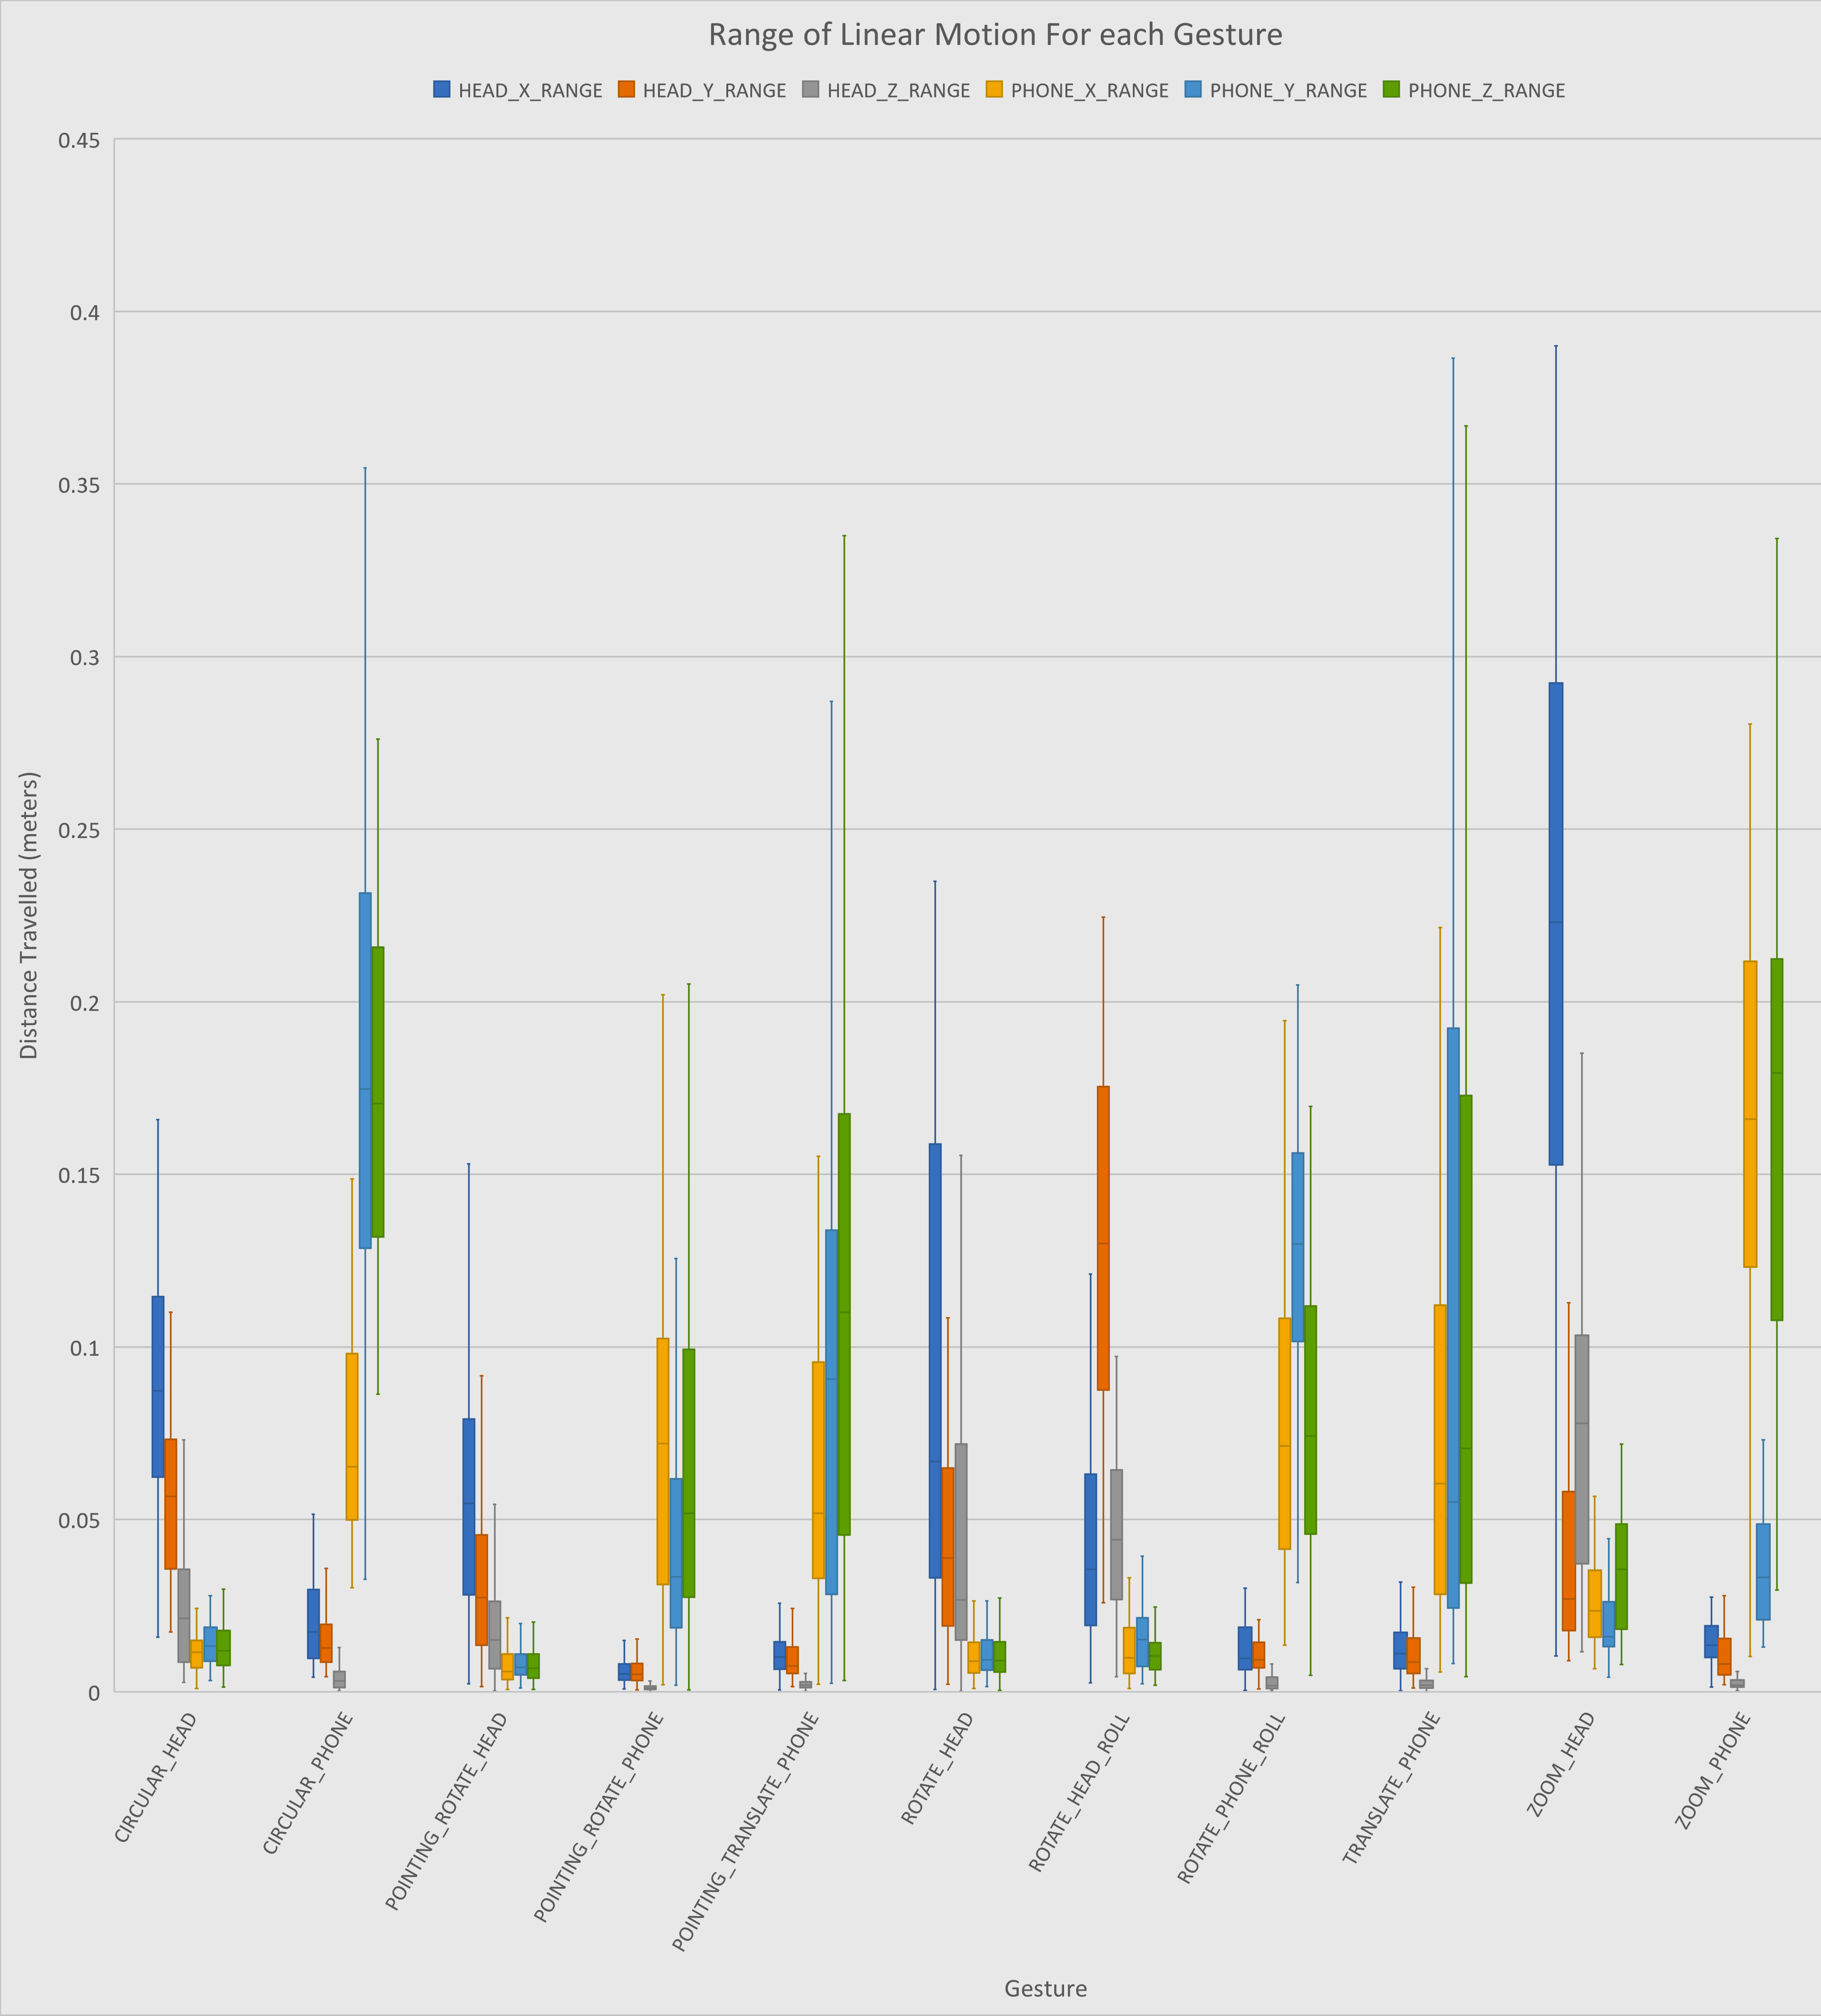
\includegraphics[width=\textwidth]{figures/RangeOfLinearMotion.png}
%     \caption{\label{fig:range_of_linear_motion} Range of linear motion for each gesture, in meters}
%     \Description{Box and Wisker plot showing the mean, min, max, and the first and third quartiles for the observed range of linear motion for each gesture recorded.}
% \end{figure}

\begin{figure}[H]
    \centering
    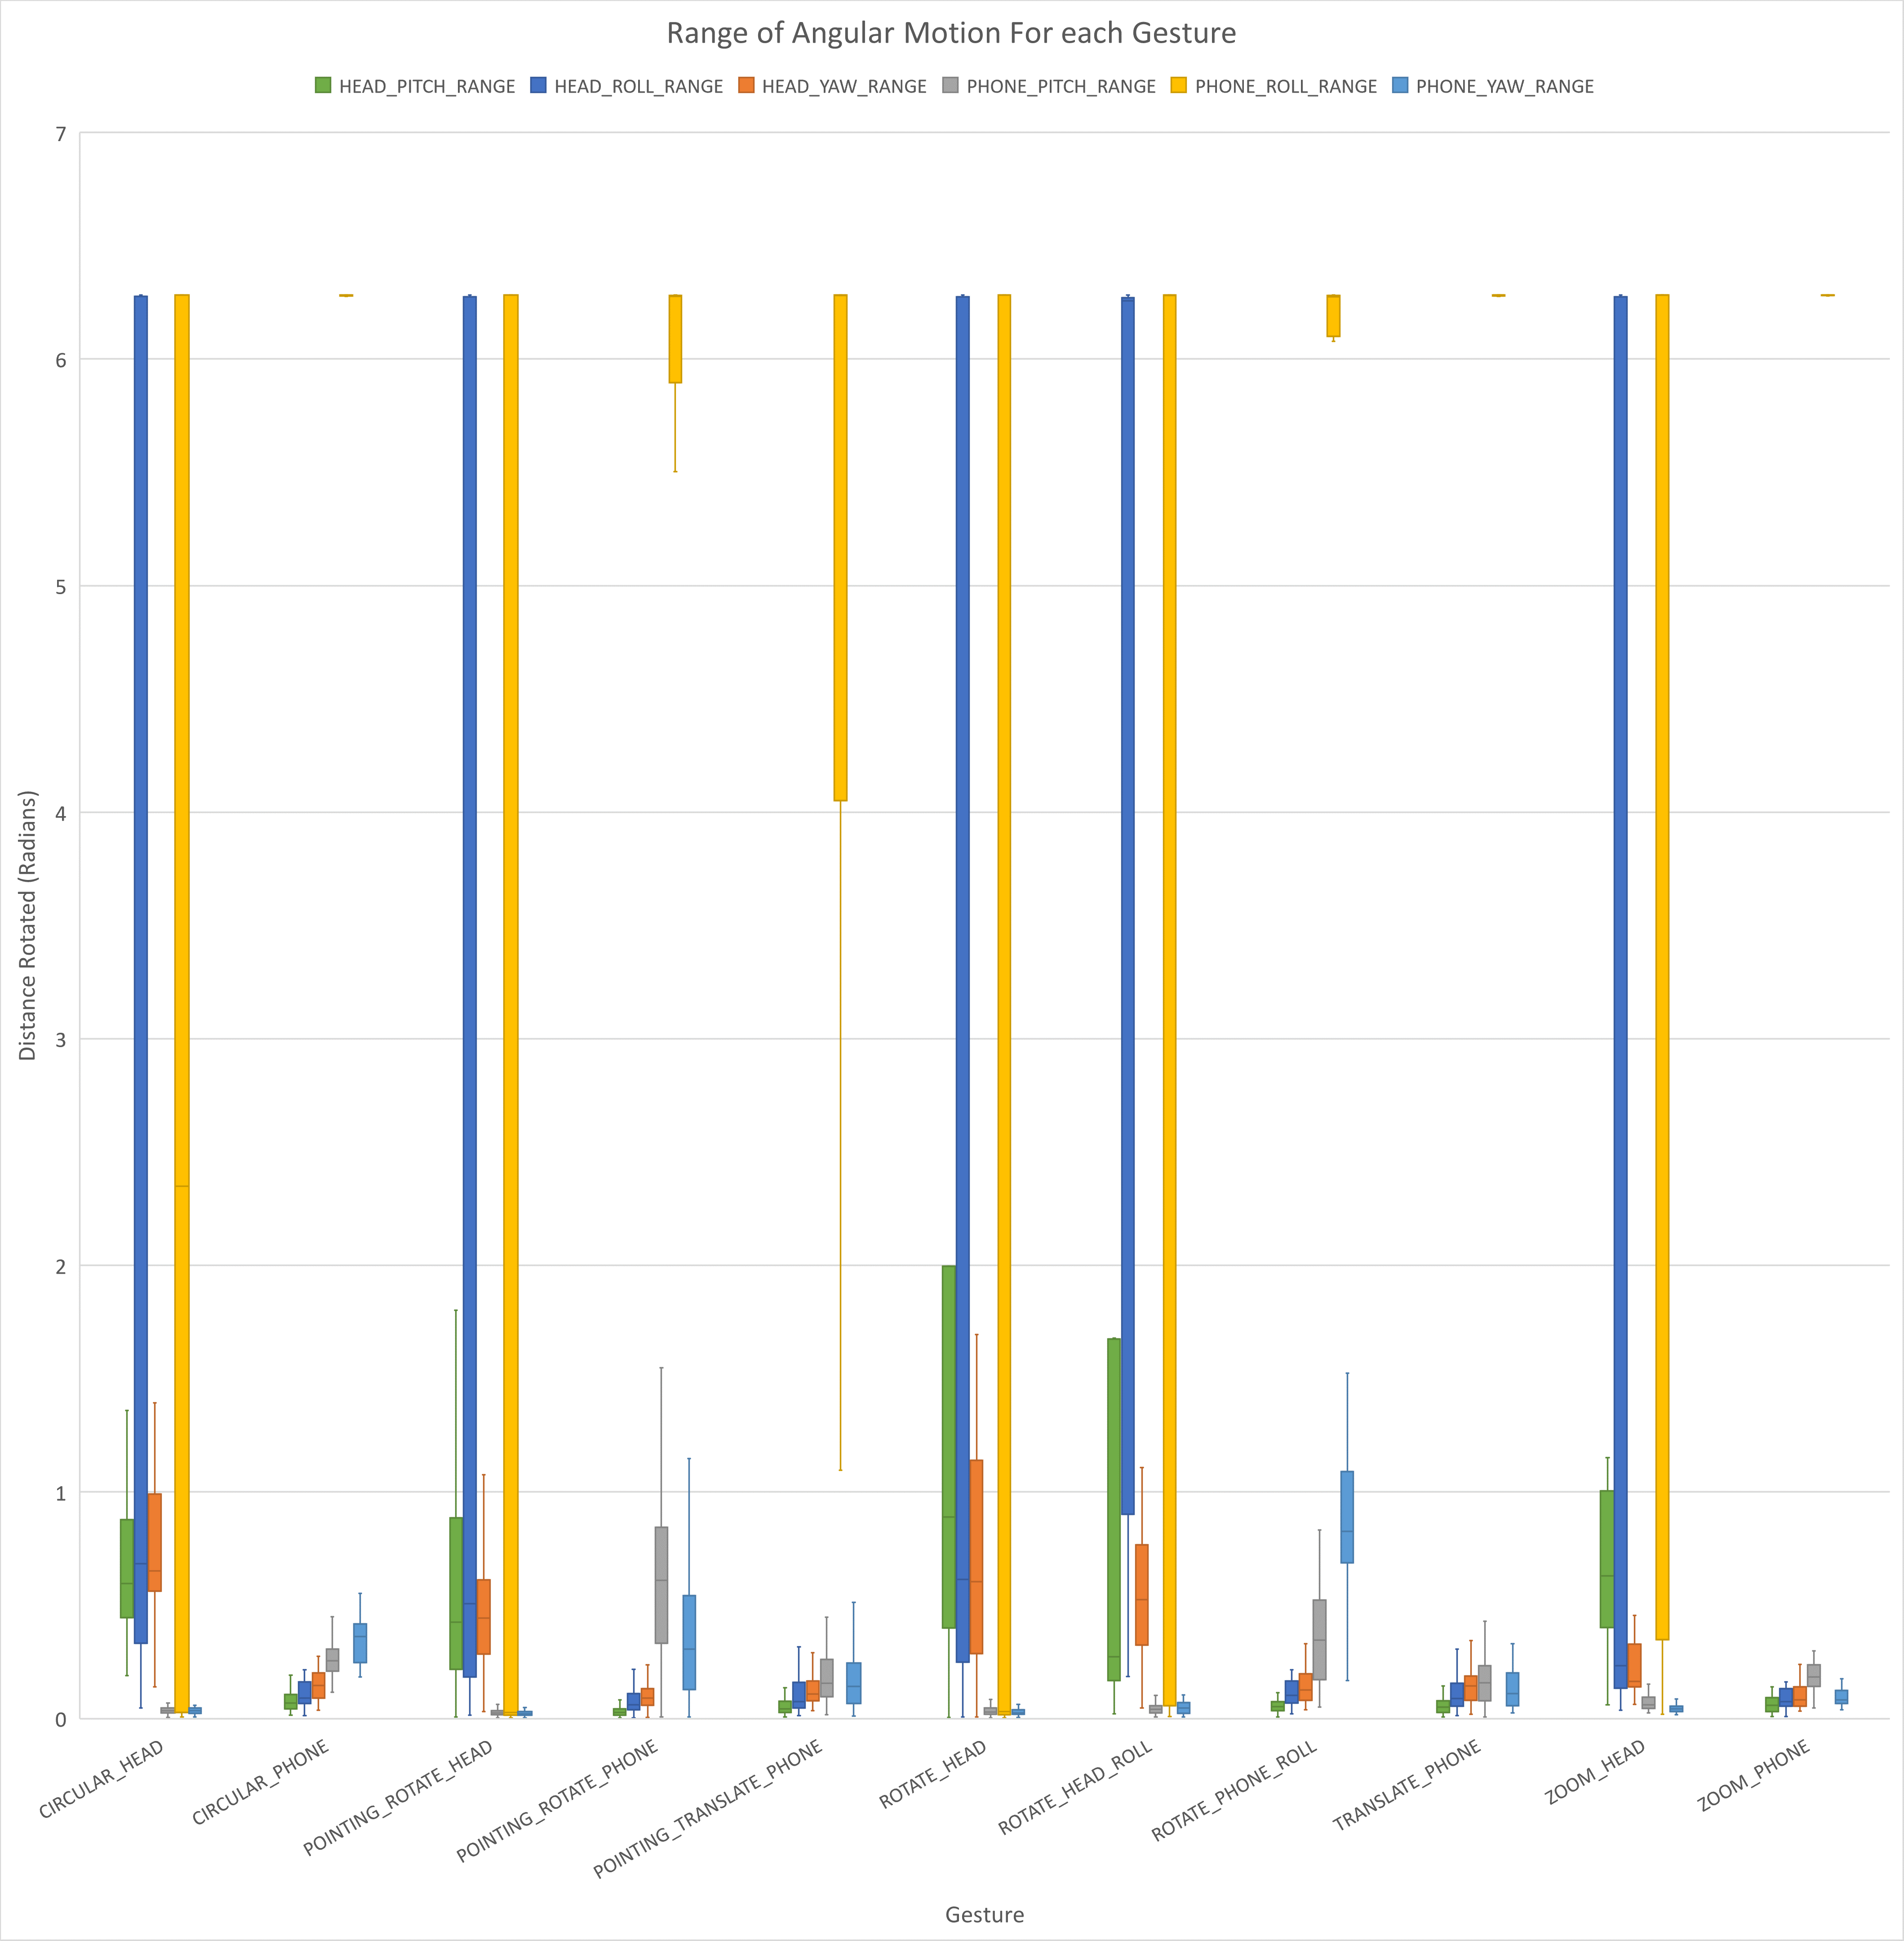
\includegraphics[width=\textwidth]{figures/RangeOfAngularMotion.png}
    \caption{\label{fig:range_of_angular_motion} Range of angular motion for each gesture, in meters}
    \Description{Box and Wisker plot showing the mean, min, max, and the first and third quartiles for the observed range of angular motion for each gesture recorded.}
\end{figure}

\newpage
\section{Code}
\subsection{Data Collection Application}
\url{https://github.com/whattheforkbomb/datacollection}

\subsection{Data Synchronisation}
\url{https://github.com/whattheforkbomb/dissertation_code/blob/trunk/datacollection/dataSynchronisation.py}

\subsection{YUV -> RGB Image Converter}
\url{https://github.com/whattheforkbomb/dissertation_code/blob/trunk/datacollection/imageGenerator.py}

\subsection{Data Resampling}
\url{https://github.com/whattheforkbomb/dissertation_code/blob/trunk/dataprocessing/data_analysis.ipynb}

\subsection{Model Development}
\url{https://github.com/whattheforkbomb/dissertation_code/blob/trunk/training/training.ipynb}

% Tell TexCount to start counting words again
%TC:endignore


\end{document}
\endinput